COMSOL Multiphysics\textsuperscript{TM} is a comprehensive software suite for finite element analysis, solving, and simulation across a wide array of physics and engineering disciplines, particularly focusing on coupled phenomena and multi-physics interactions. It enables the creation and simulation of physics-based models and applications in an intuitive, interactive workspace.

COMSOL software supports a broad spectrum of applications, from electromagnetics and structural mechanics to acoustics, fluid dynamics, heat transfer, and chemical engineering. COMSOL features an extensive array of modules, including the Wave Optics module for optical applications simulations like wave propagation in fiber optics and photonics, the Semiconductor module for the analysis of semiconductor devices such as diodes and transistors, and the AC/DC module for examining electric and magnetic fields in static and low-frequency scenarios.

For my thesis, which involves analyzing ray paths in optical systems, I will be utilizing the Ray Optics module.

% ----- THE MODELLING WORKFLOW -----
\section{The COMSOL Modelling Workflow}
Briefly the modelling workflow consists of the following steps; illustrated in Figure \ref{fig:The modeling workflow.}, if you start a model completely from scratch:

\begin{enumerate}
    \item \textbf{Initialization of the Model Environment}: Preparing the foundational settings for the simulation.
    \item \textbf{Geometry Construction}: Designing the model's physical layout.
    \item \textbf{Material Property Specification}: Assigning specific materials to the model components.
    \item \textbf{Physics Boundary Conditions Definition}: Establishing the physical constraints and conditions.
    \item \textbf{Mesh Generation}: Creating the computational grid over the model.
    \item \textbf{Simulation Execution}: Performing the actual computational analysis.
    \item \textbf{Results Post-Processing}: Analyzing and visualizing the simulation outcomes.
\end{enumerate}

% COMSOL Modelling workflow
\begin{figure}[H]
  \centering
  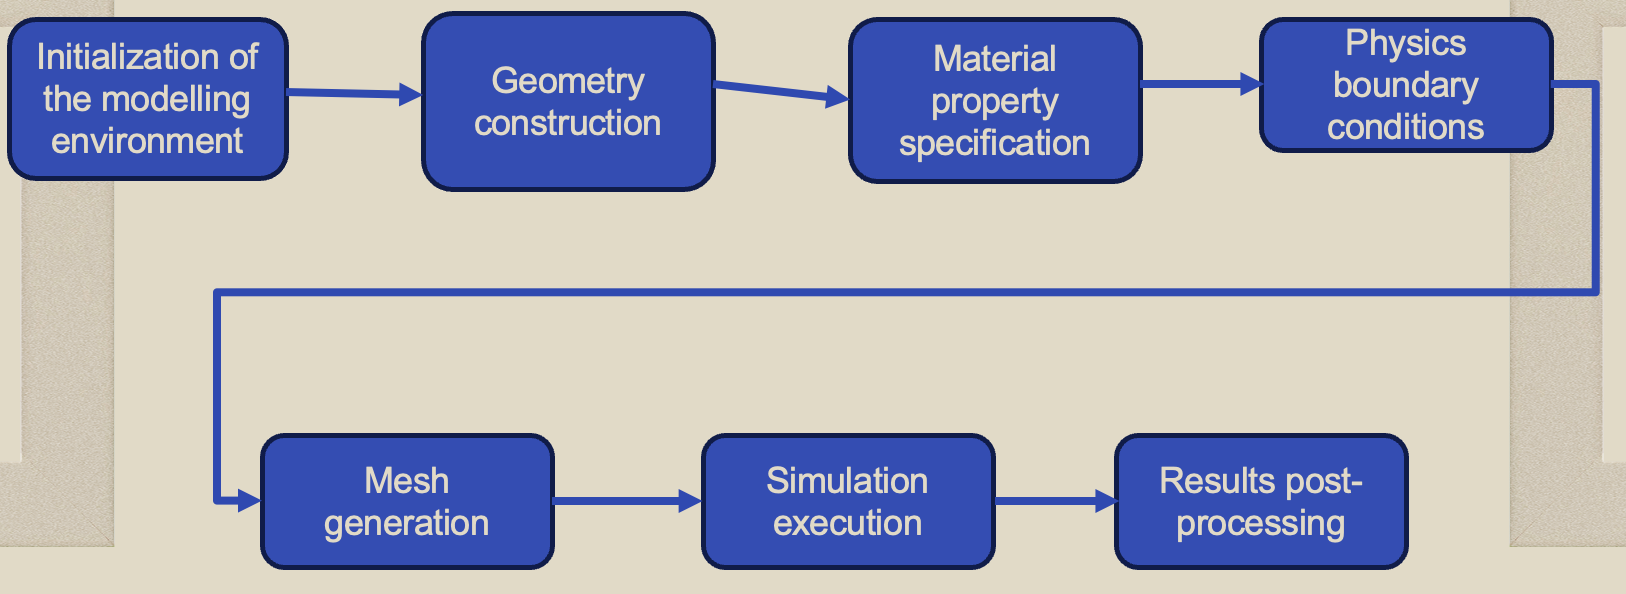
\includegraphics[width=0.7\textwidth]{Chapters/Figures/Chapter 3 Figures/COMSOL Modelling Workflow.png}
  \caption{The modeling workflow.}
  \label{fig:The modeling workflow.}
\end{figure}

In this context, I will demonstrate this workflow first through a simple project, illustrating COMSOL's robust capabilities and the straightforwardness of applying this workflow across various projects, following the sample tutorial given in \cite{multiphysics__modeling_nodate}. It's important to recognize that this workflow remains consistent across different physics simulations, which will guide the development of subsequent models for my thesis.

This demonstration will focus on simulating Joule heating within a busbar, a process where electric current passing through metal results in heating due to electrical resistance.

The busbar in question will incorporate three titanium bolts, with electrical current flowing from a single bolt on one end to a pair of bolts at the opposite end. The objective is to observe the resulting temperature distribution as the busbar undergoes heating.

% Busbar image
\begin{figure}[H]
  \centering
  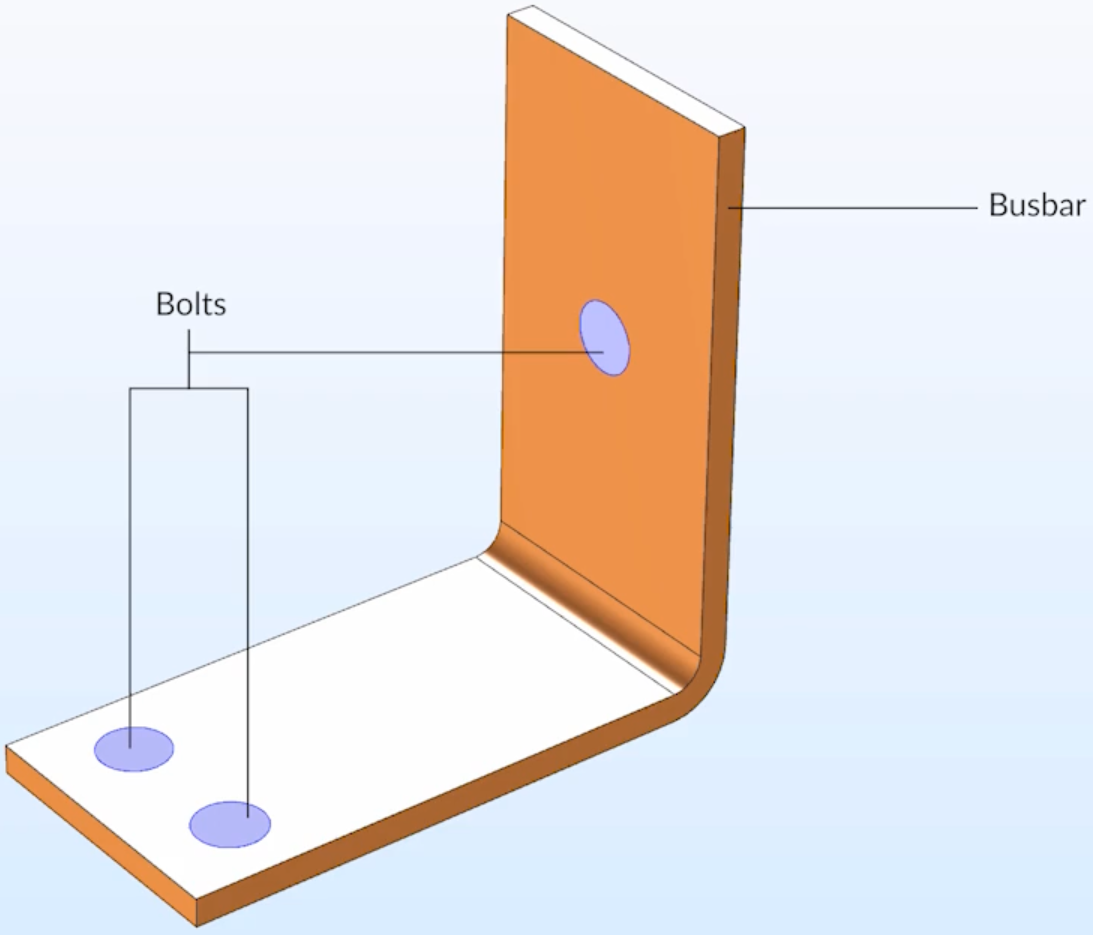
\includegraphics[width=0.7\textwidth]{Chapters/Figures/Chapter 3 Figures/Busbar.png}
  \caption{The busbar model. Source: \cite{multiphysics__modeling_nodate}}
  \label{fig:The busbar model}
\end{figure}

% SUBSECTION --- Setting up the model environment ---
\subsection{Setting Up the Model Environment}.
% TODO: Add set-up screen image
\begin{figure}[H]
  \centering
  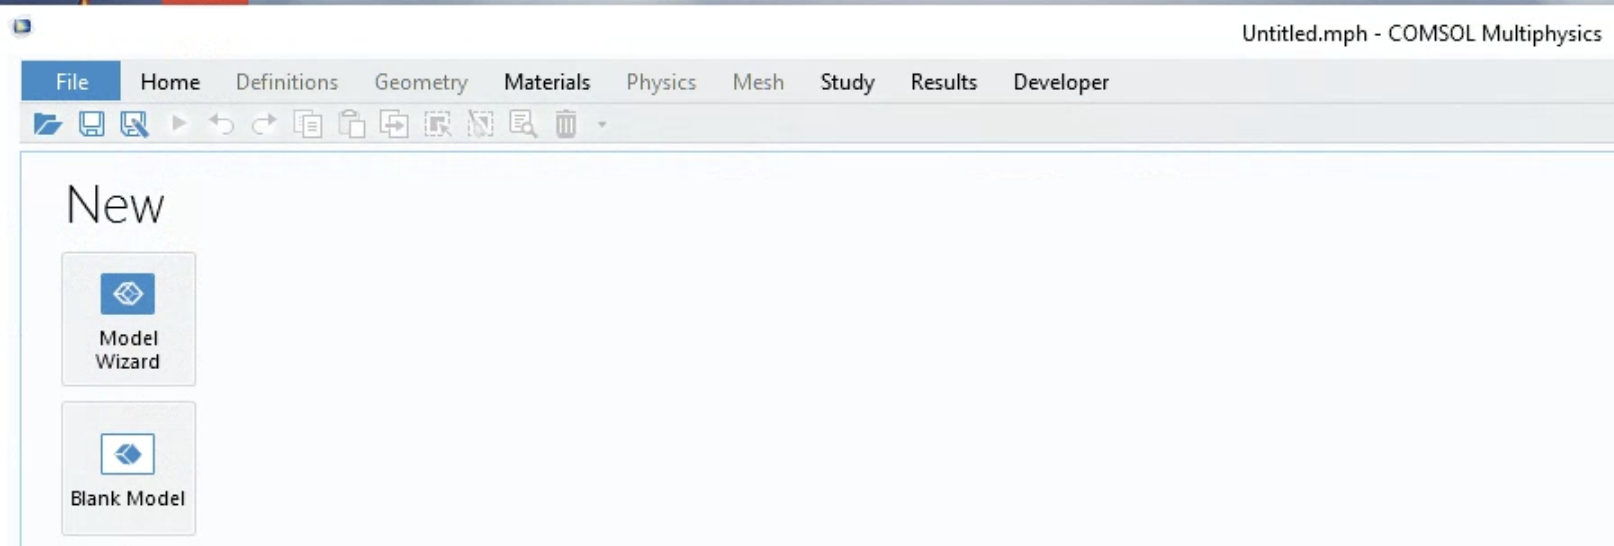
\includegraphics[width=0.7\textwidth]{Chapters/Figures/Chapter 3 Figures/Set-up Screen.png}
  \caption{Set-up Screen. Source: \cite{multiphysics__modeling_nodate}}
  \label{fig:Set-up Screen}
\end{figure}

Upon launching COMSOL, you are presented with an option to initiate a new project: selecting a Blank Model for starting anew or opting for the Model Wizard for a guided setup. The Model Wizard is advisable for its structured selection process integral to configuring your model. Conversely, choosing a Blank Model grants immediate access to the COMSOL desktop interface, bypassing the preliminary selections required by the Model Wizard.

% TODO: Add "Select Space Dimension" image
\begin{figure}[H]
  \centering
  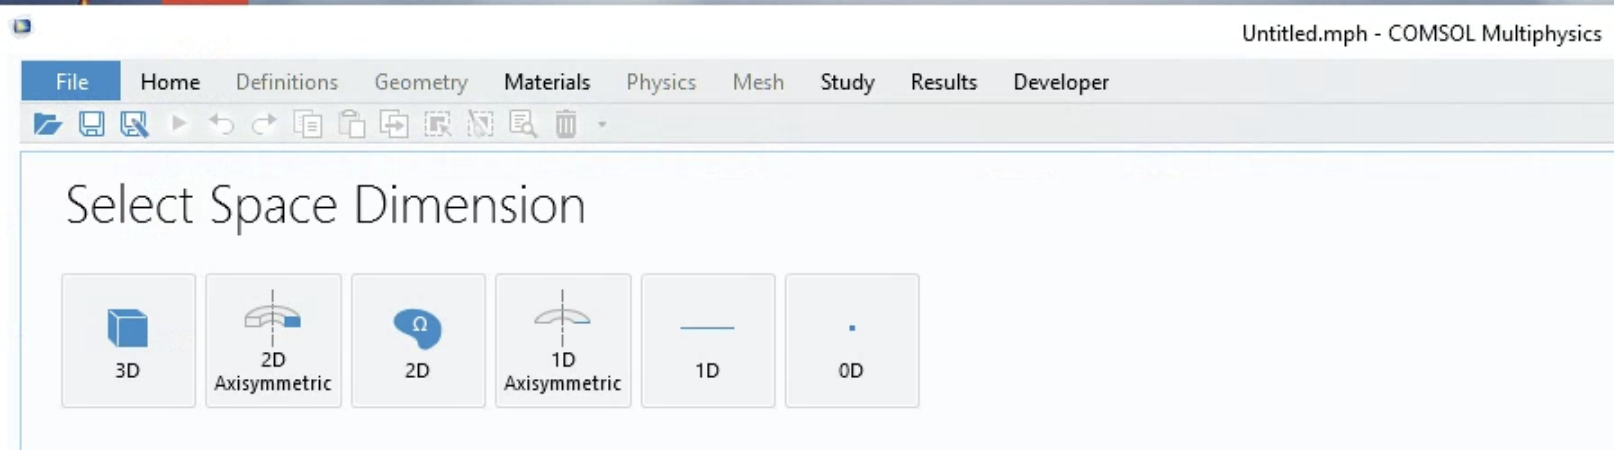
\includegraphics[width=0.7\textwidth]{Chapters/Figures/Chapter 3 Figures/Select Space Dimension.png}
  \caption{Select space dimension screen. Source: \cite{multiphysics__modeling_nodate}}
  \label{fig:Select Space Dimension}
\end{figure}

Since our busbar model requires a three-dimensional framework, I select the ``3D'' option.

% TODO: Add "Select Physics" image
\begin{figure}[H]
  \centering
  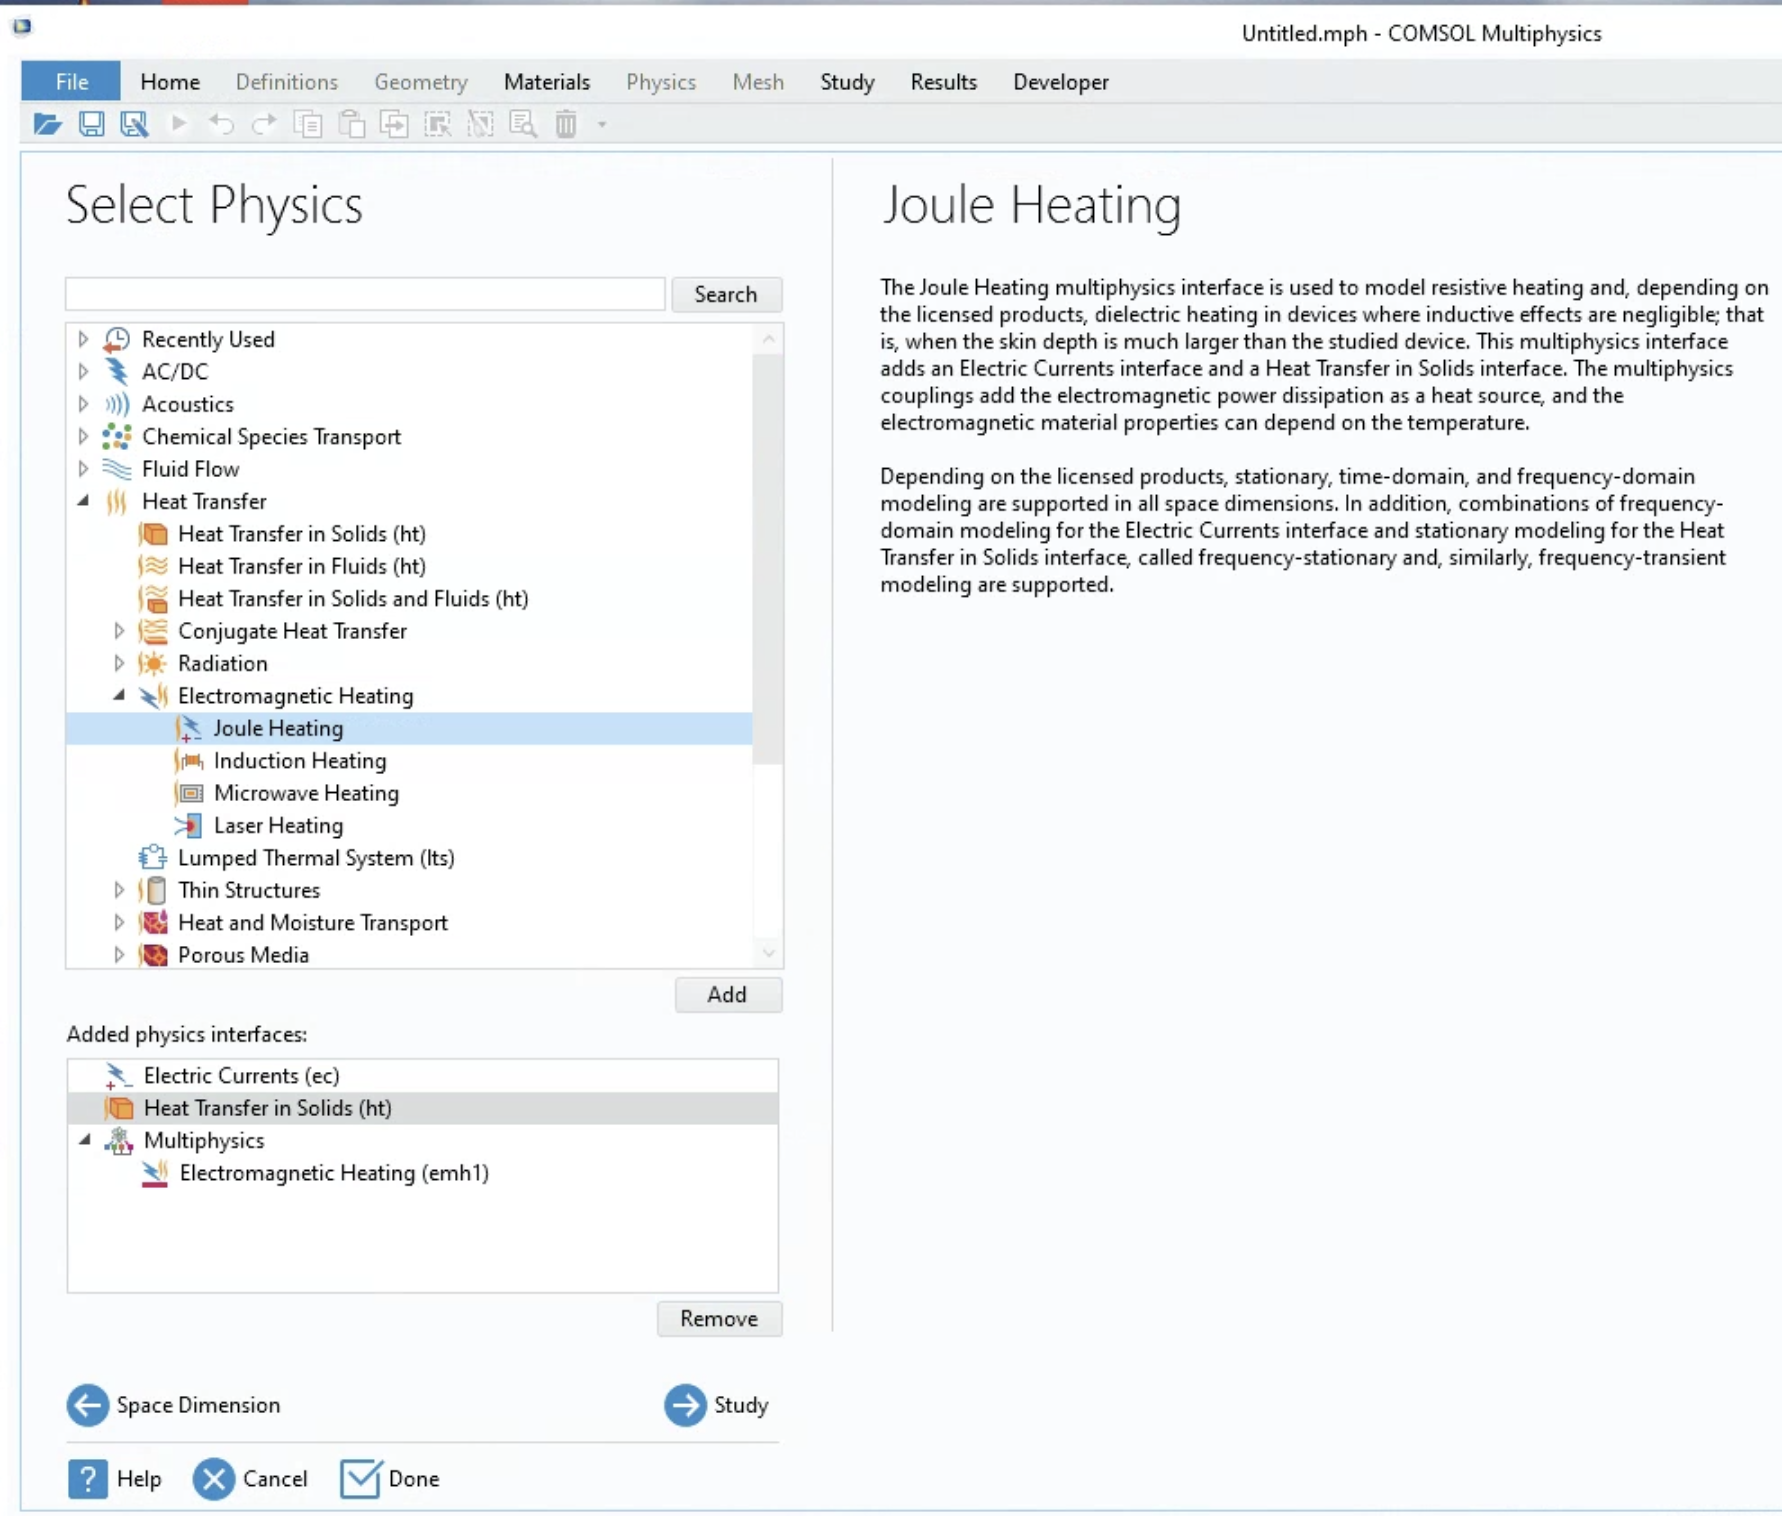
\includegraphics[width=0.7\textwidth]{Chapters/Figures/Chapter 3 Figures/Select Physics.png}
  \caption{Select physics screen. Source: \cite{multiphysics__modeling_nodate}}
  \label{fig:Select Physics}
\end{figure}

Subsequently, I arrive at a prompt to select the desired physics for the model. In our case, I opt for Joule heating. In another scenario, for instance, if one's project was on thin-film fluid flow, navigating to the ``Fluid Flow'' node and selecting ``Thin-Film Flow'' would be the procedure. Adding ``Joule Heating'' automatically associates it with related physics categories like ``Electric Currents (ec)'' and ``Heat Transfer in Solids (ht),'' indicating that ``Joule Heating'' encompasses a composite interface with multiple physics elements integrated.

The selection of physics for exploration significantly hinges on the project's specific requirements and the level of access provided by your COMSOL subscription. For example, acquiring the ``Ray Optics'' module necessary for my thesis entailed a waiting period due to initial subscription limitations. Therefore, early verification of the required physics modules for your project is recommended.

To proceed, I select ``Study''.

% TODO: Add "Select Study" image
\begin{figure}[H]
  \centering
  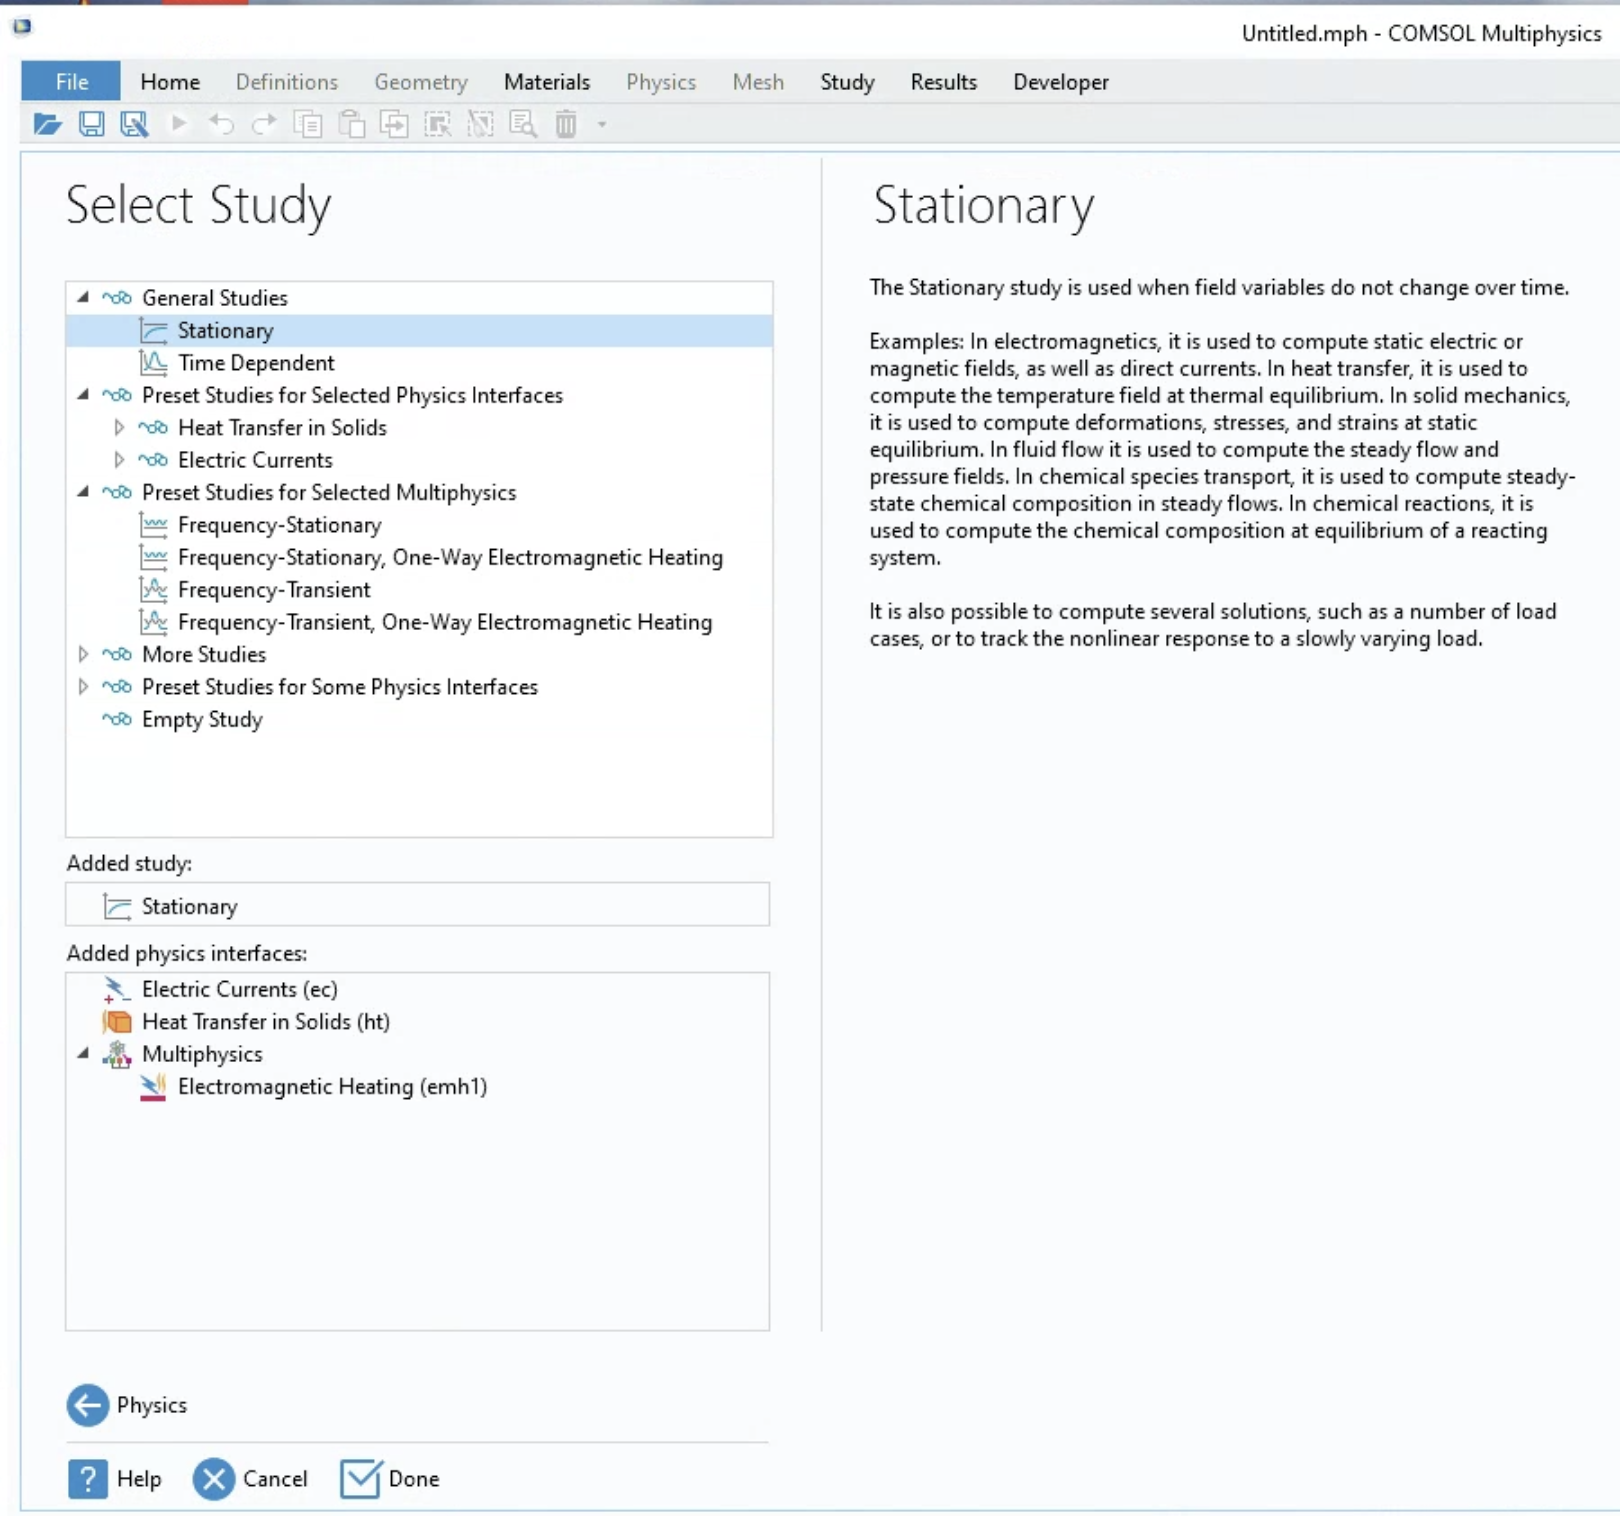
\includegraphics[width=0.7\textwidth]{Chapters/Figures/Chapter 3 Figures/Select Study.png}
  \caption{Select study screen. Source: \cite{multiphysics__modeling_nodate}}
  \label{fig:Select Study}
\end{figure}

Upon accessing this interface, I am presented with an assortment of study options, determined by our earlier selections regarding the model's spatial dimensions and physics. For our busbar analysis, the ``Stationary'' study suffices, given its static nature. After selecting ``Done'', I transition to the COMSOL desktop environment.

% TODO: Add "COMSOL Desktop" image
\begin{figure}[H]
  \centering
  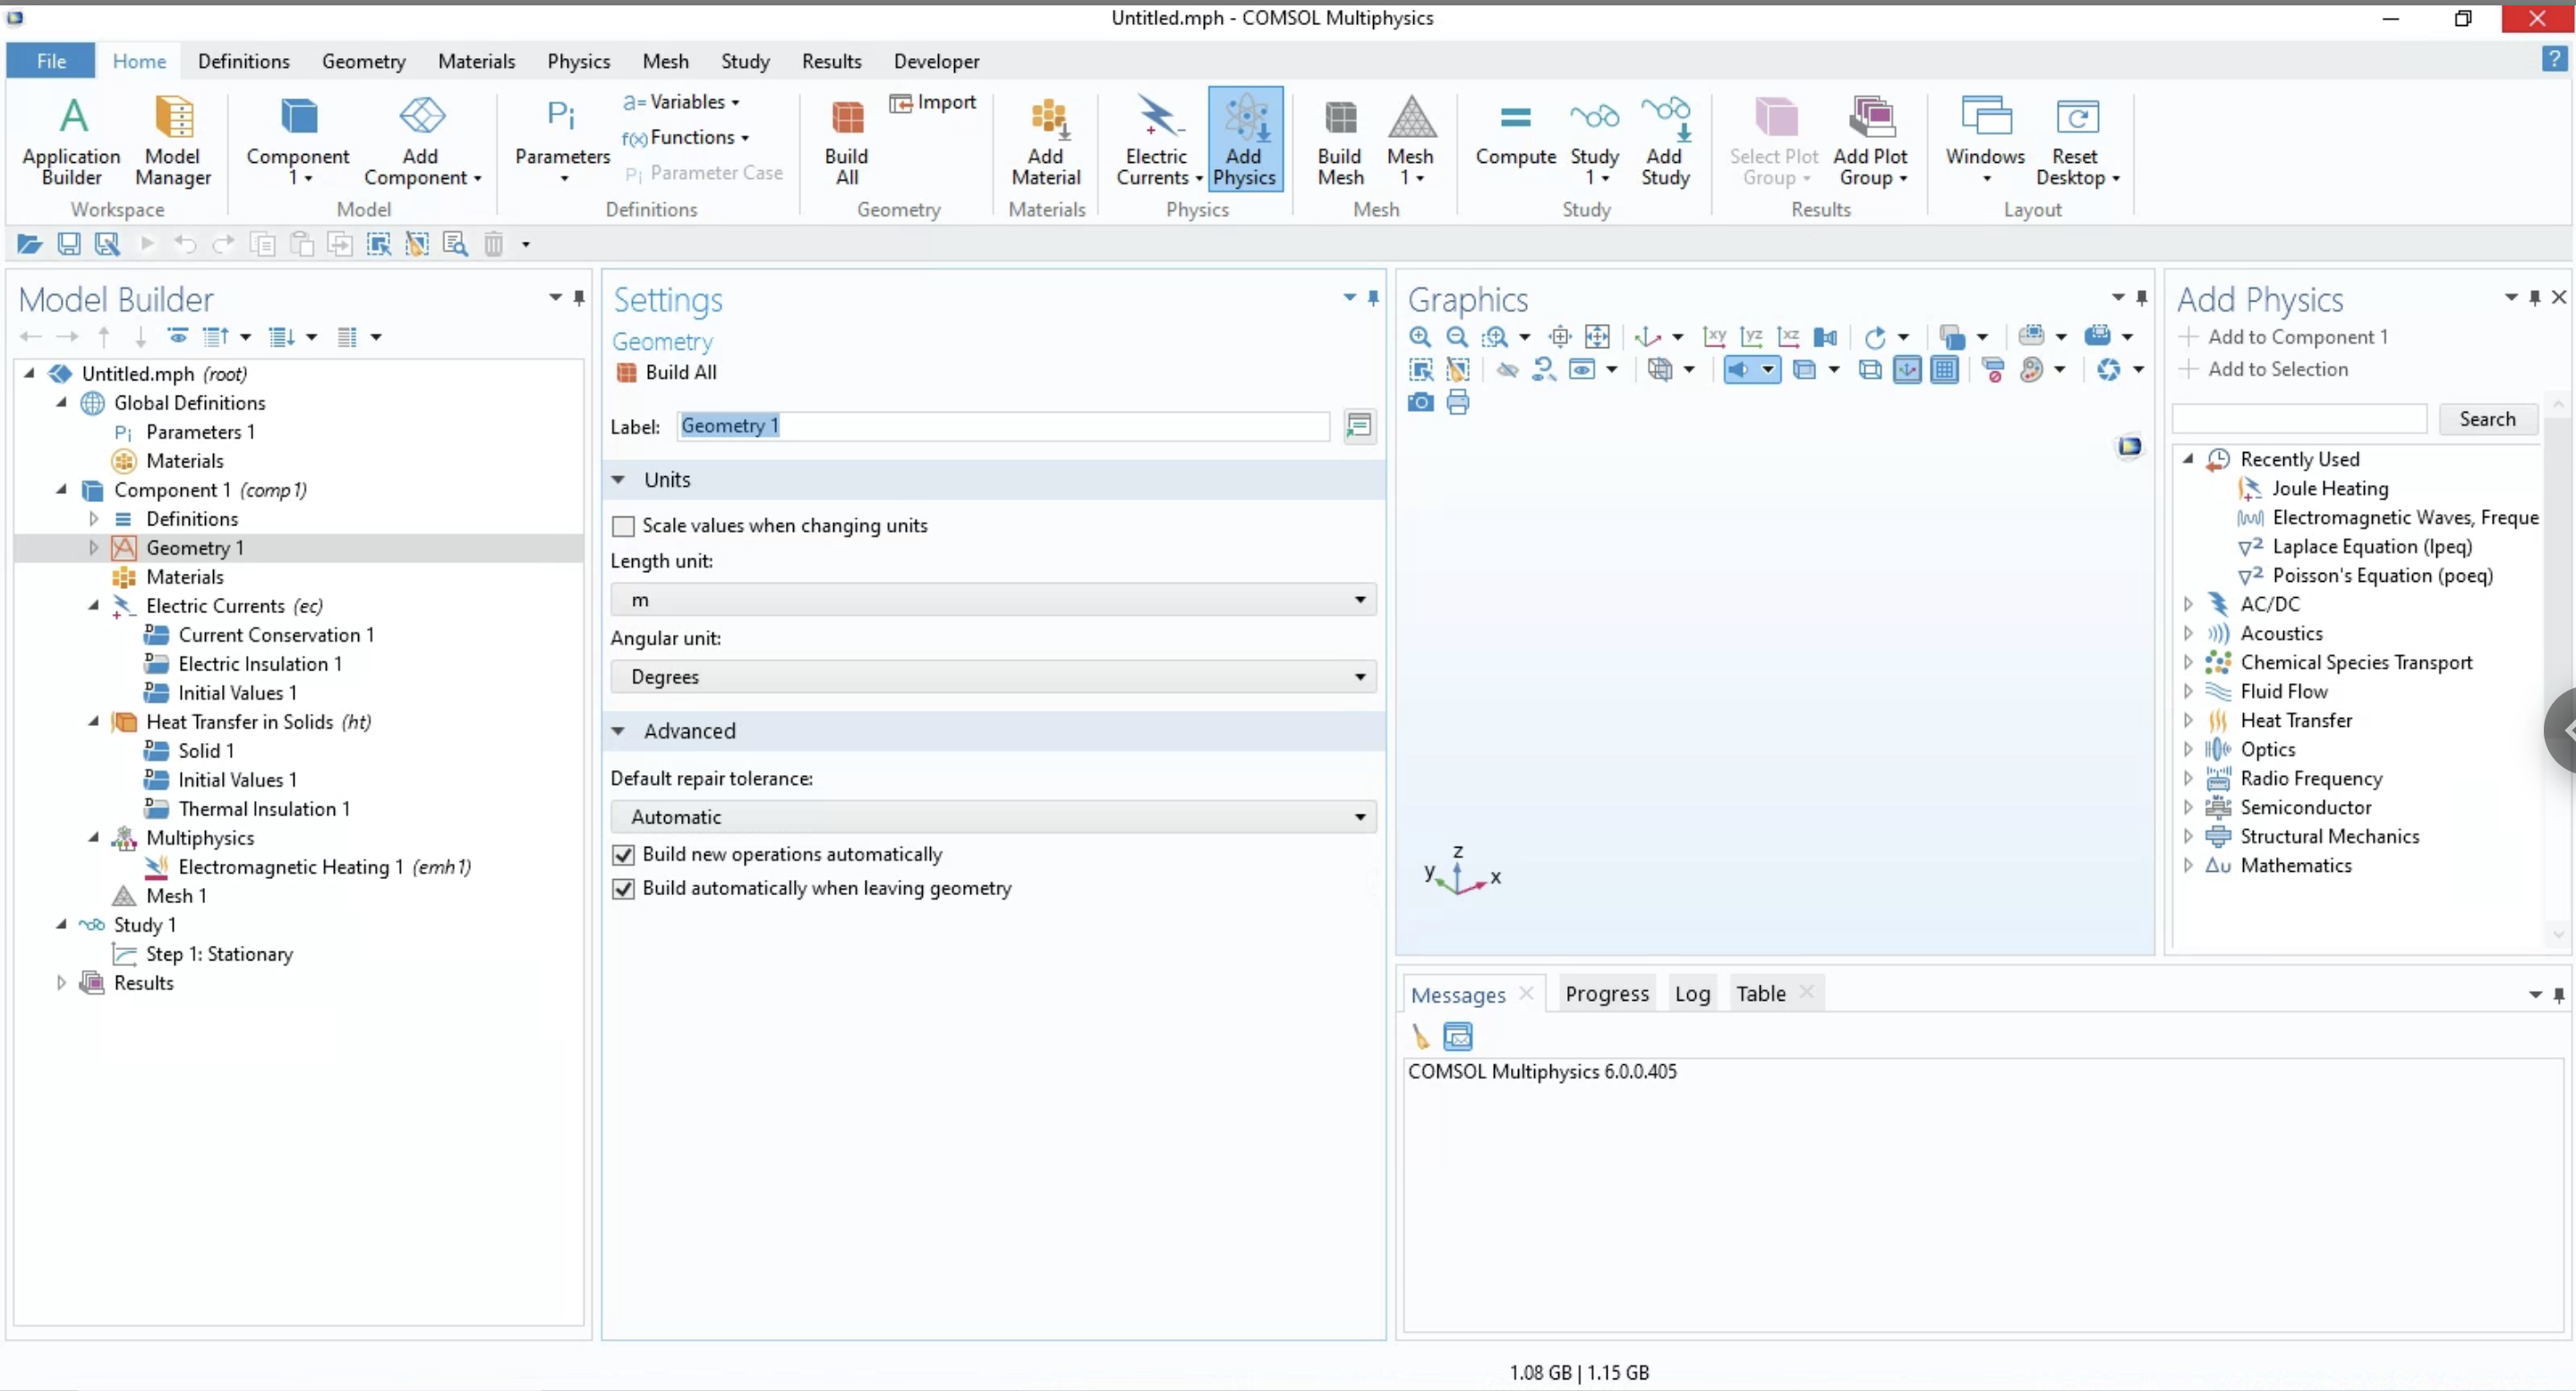
\includegraphics[width=0.7\textwidth]{Chapters/Figures/Chapter 3 Figures/Initial COMSOL Desktop.png}
  \caption{The COMSOL desktop. Source: \cite{multiphysics__modeling_nodate}}
  \label{fig:The COMSOL desktop}
\end{figure}

The COMSOL desktop serves as the central hub for constructing and engaging with your model from the ground up. It is designed with an intuitive interface, featuring buttons and ribbons aligned with the modeling process steps. Within the Model Builder window, you'll find the modeling hierarchy, where you have the capability to define your model's dimensions and select specific physics equations for adherence. Additionally, the layout of the COMSOL desktop windows can be customized to suit your preferences.

% SUBSECTION --- Building the Geometry ---
\subsection{Building the Geometry}.
When developing the geometry of your model, multiple pathways are available. You may opt to utilize the drawing tools or geometric shapes provided by COMSOL or import a geometry from an external source.

% TODO: Add "Geometry Button" image
\begin{figure}[H]
  \centering
  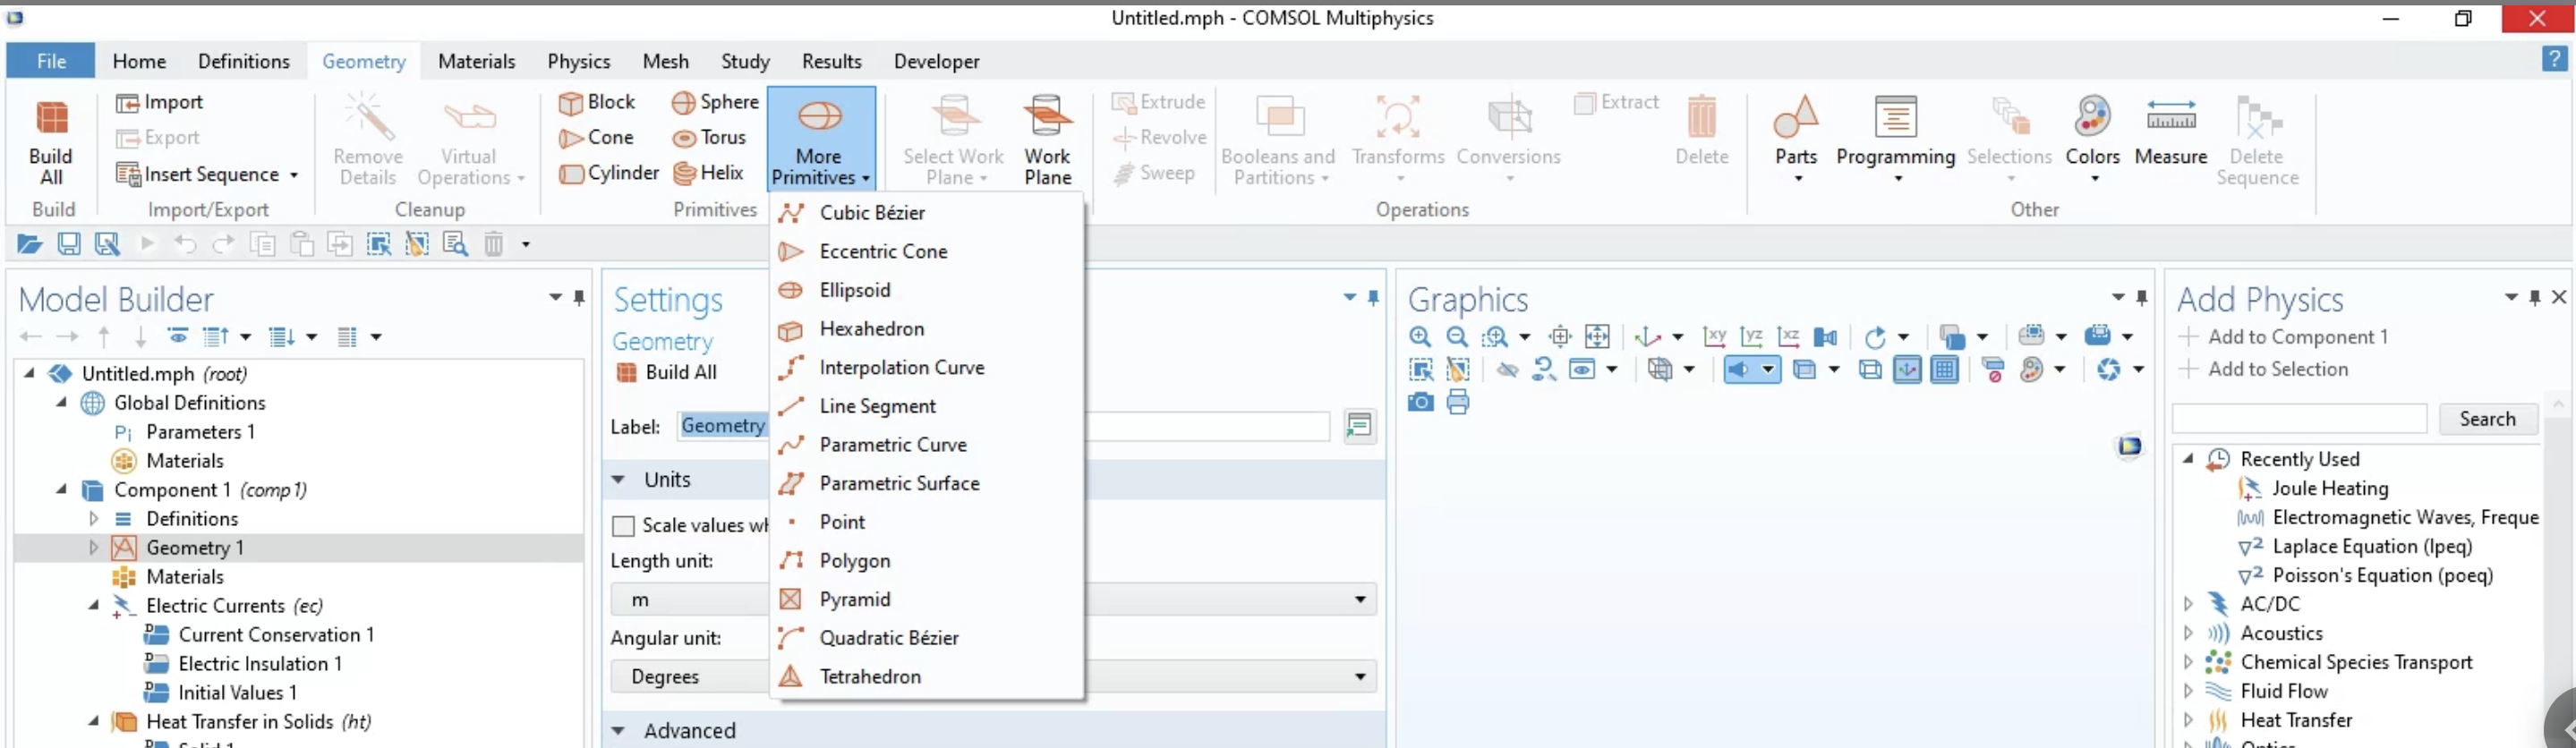
\includegraphics[width=0.7\textwidth]{Chapters/Figures/Chapter 3 Figures/Geometry Tab.png}
  \caption{Add geometry button selection. Source: \cite{multiphysics__modeling_nodate}}
  \label{fig:Add geometry button selection.}
\end{figure}

For this instance, given that the busbar geometry already exists within COMSOL's comprehensive library of pre-configured geometries, accessing this resource simplifies the process. This is achieved by navigating to the File menu and selecting Application Libraries.

% TODO: Add image containing "application libraries" selection
\begin{figure}[H]
  \centering
  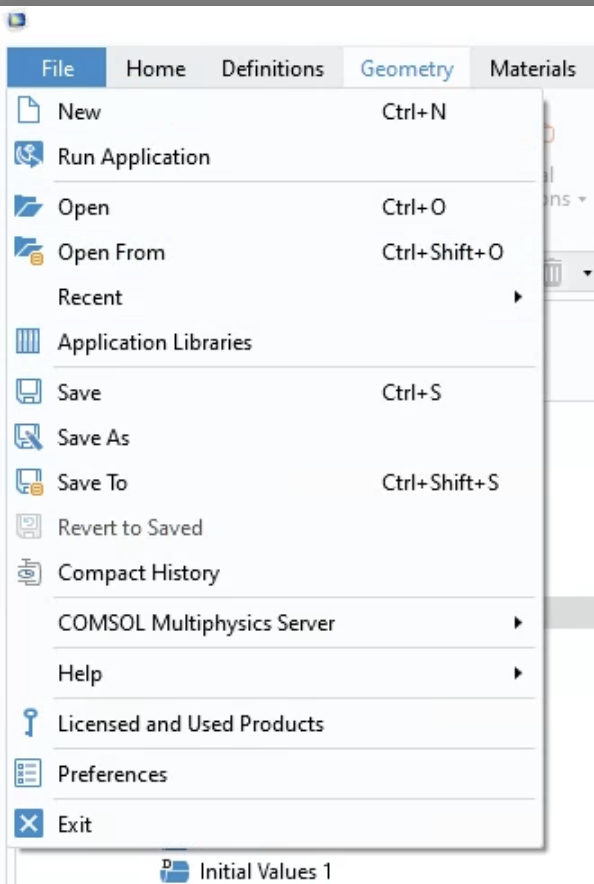
\includegraphics[width=0.7\textwidth]{Chapters/Figures/Chapter 3 Figures/Application Libraries Button.png}
  \caption{Application libraries selection. Source: \cite{multiphysics__modeling_nodate}}
  \label{fig:"application libraries" selection}
\end{figure}

Within the Application Libraries, proceed to the COMSOL Multiphysics section, locate the 'busbar\_geom' file, open it, and proceed to save your project accordingly.

% TODO: Add "Application Libraries" image
\begin{figure}[H]
  \centering
  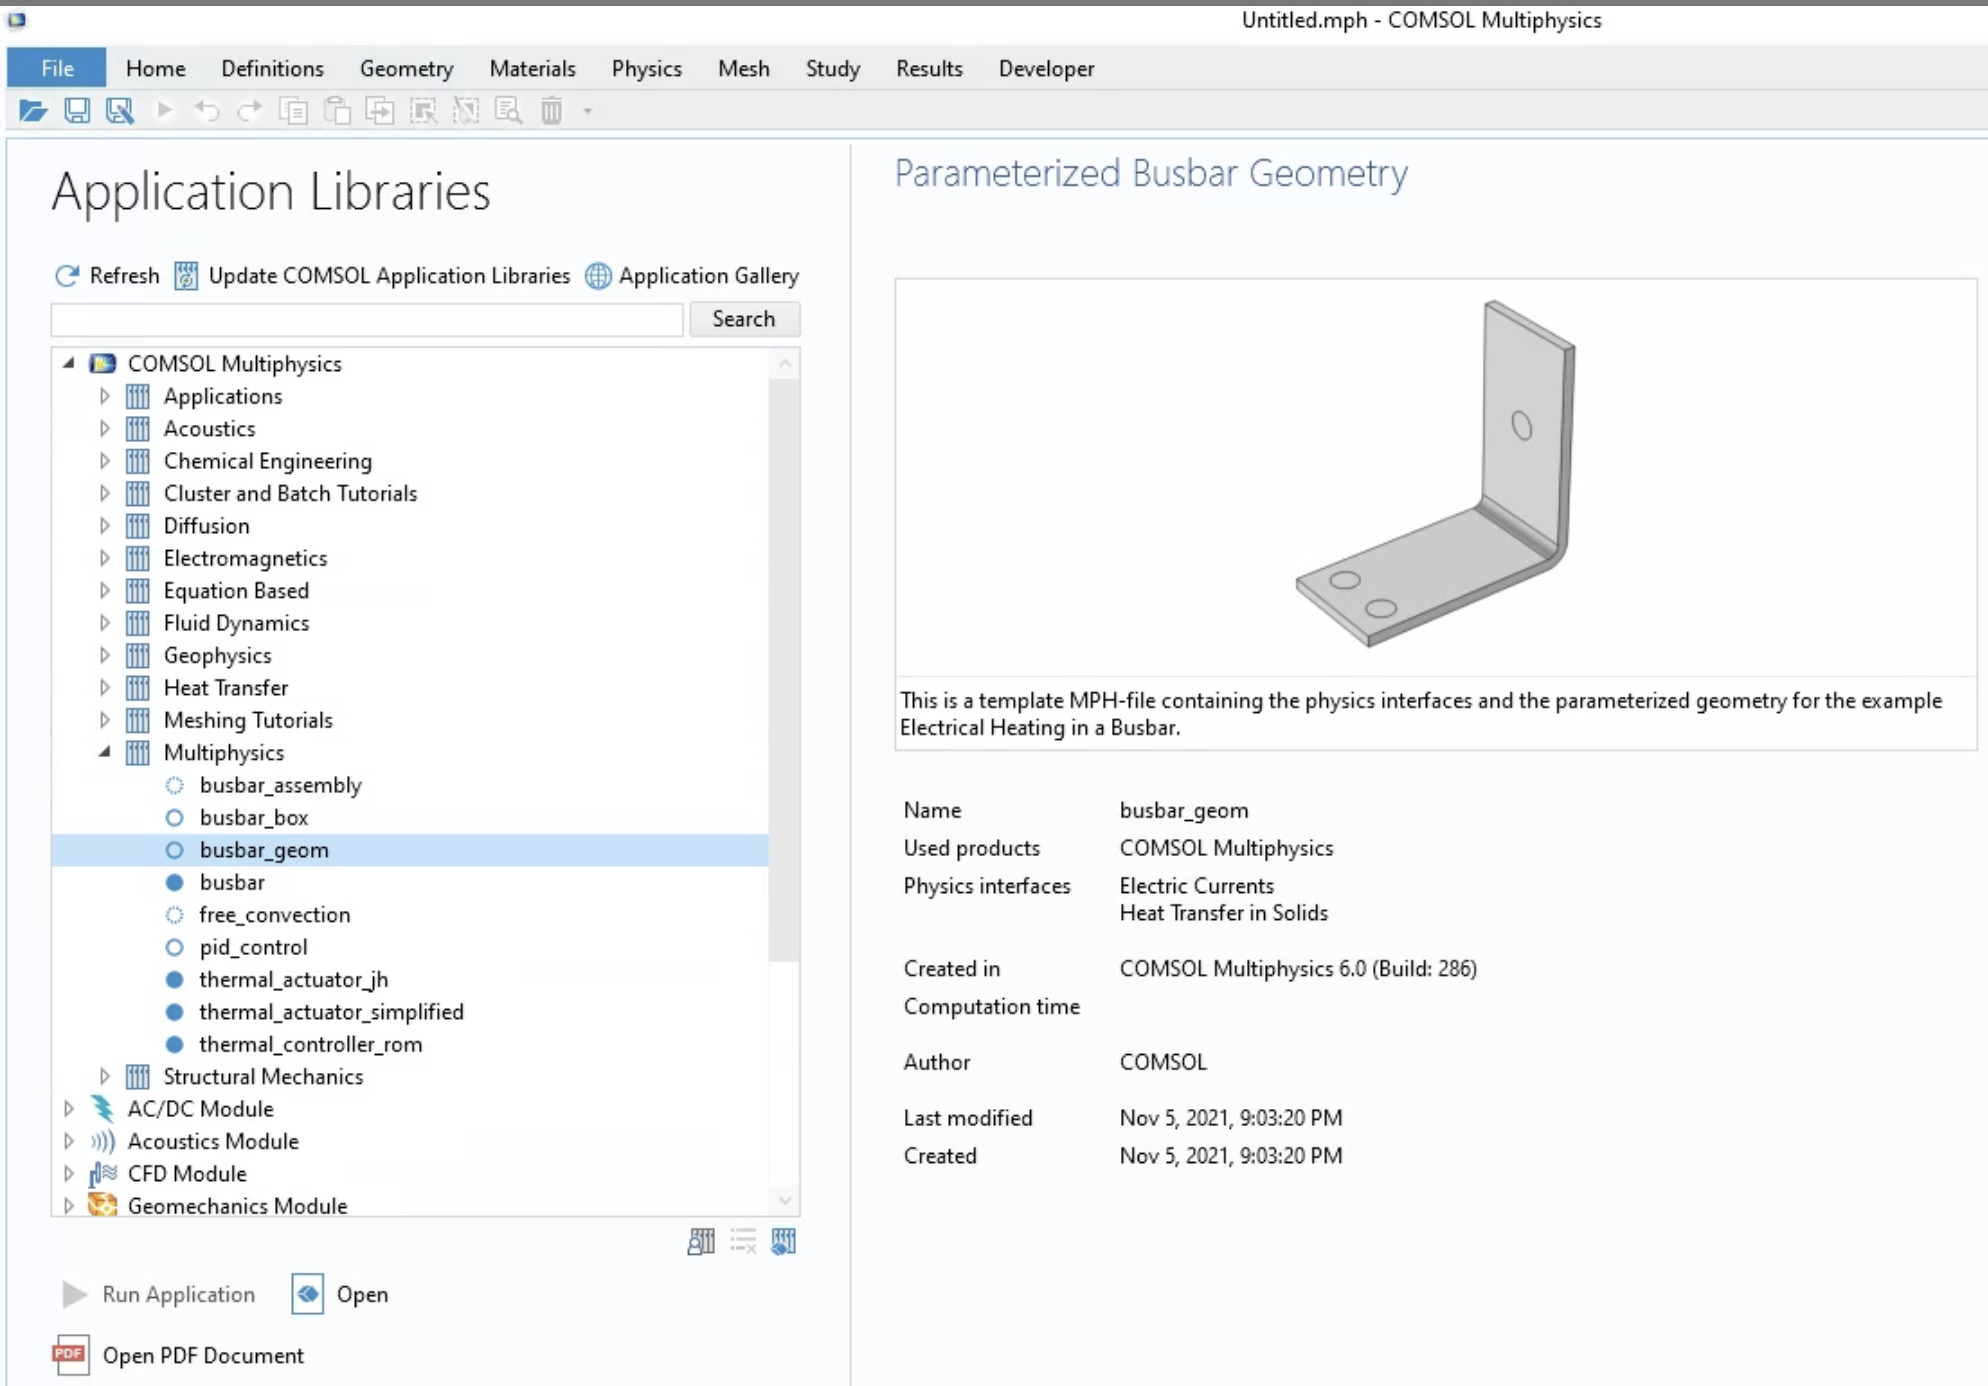
\includegraphics[width=0.7\textwidth]{Chapters/Figures/Chapter 3 Figures/Application Libraries.png}
  \caption{Application libraries. Source: \cite{multiphysics__modeling_nodate}}
  \label{fig:Application libraries}
\end{figure}

The geometry will now appear in the Graphics window, allowing for zoom and rotational exploration to closely inspect the model. The alteration in the Geometry node within the Model Builder window reflects the sequence of actions executed to construct the busbar geometry. On closer inspection, it becomes evident that specific parameters were employed in crafting this geometry. These parameters are accessible within the ``Parameters 1'' node, which contains a table detailing the adjustable parameters utilized in the geometry's creation.

% TODO: Add image after when you add default busbar geom to model
\begin{figure}[H]
  \centering
  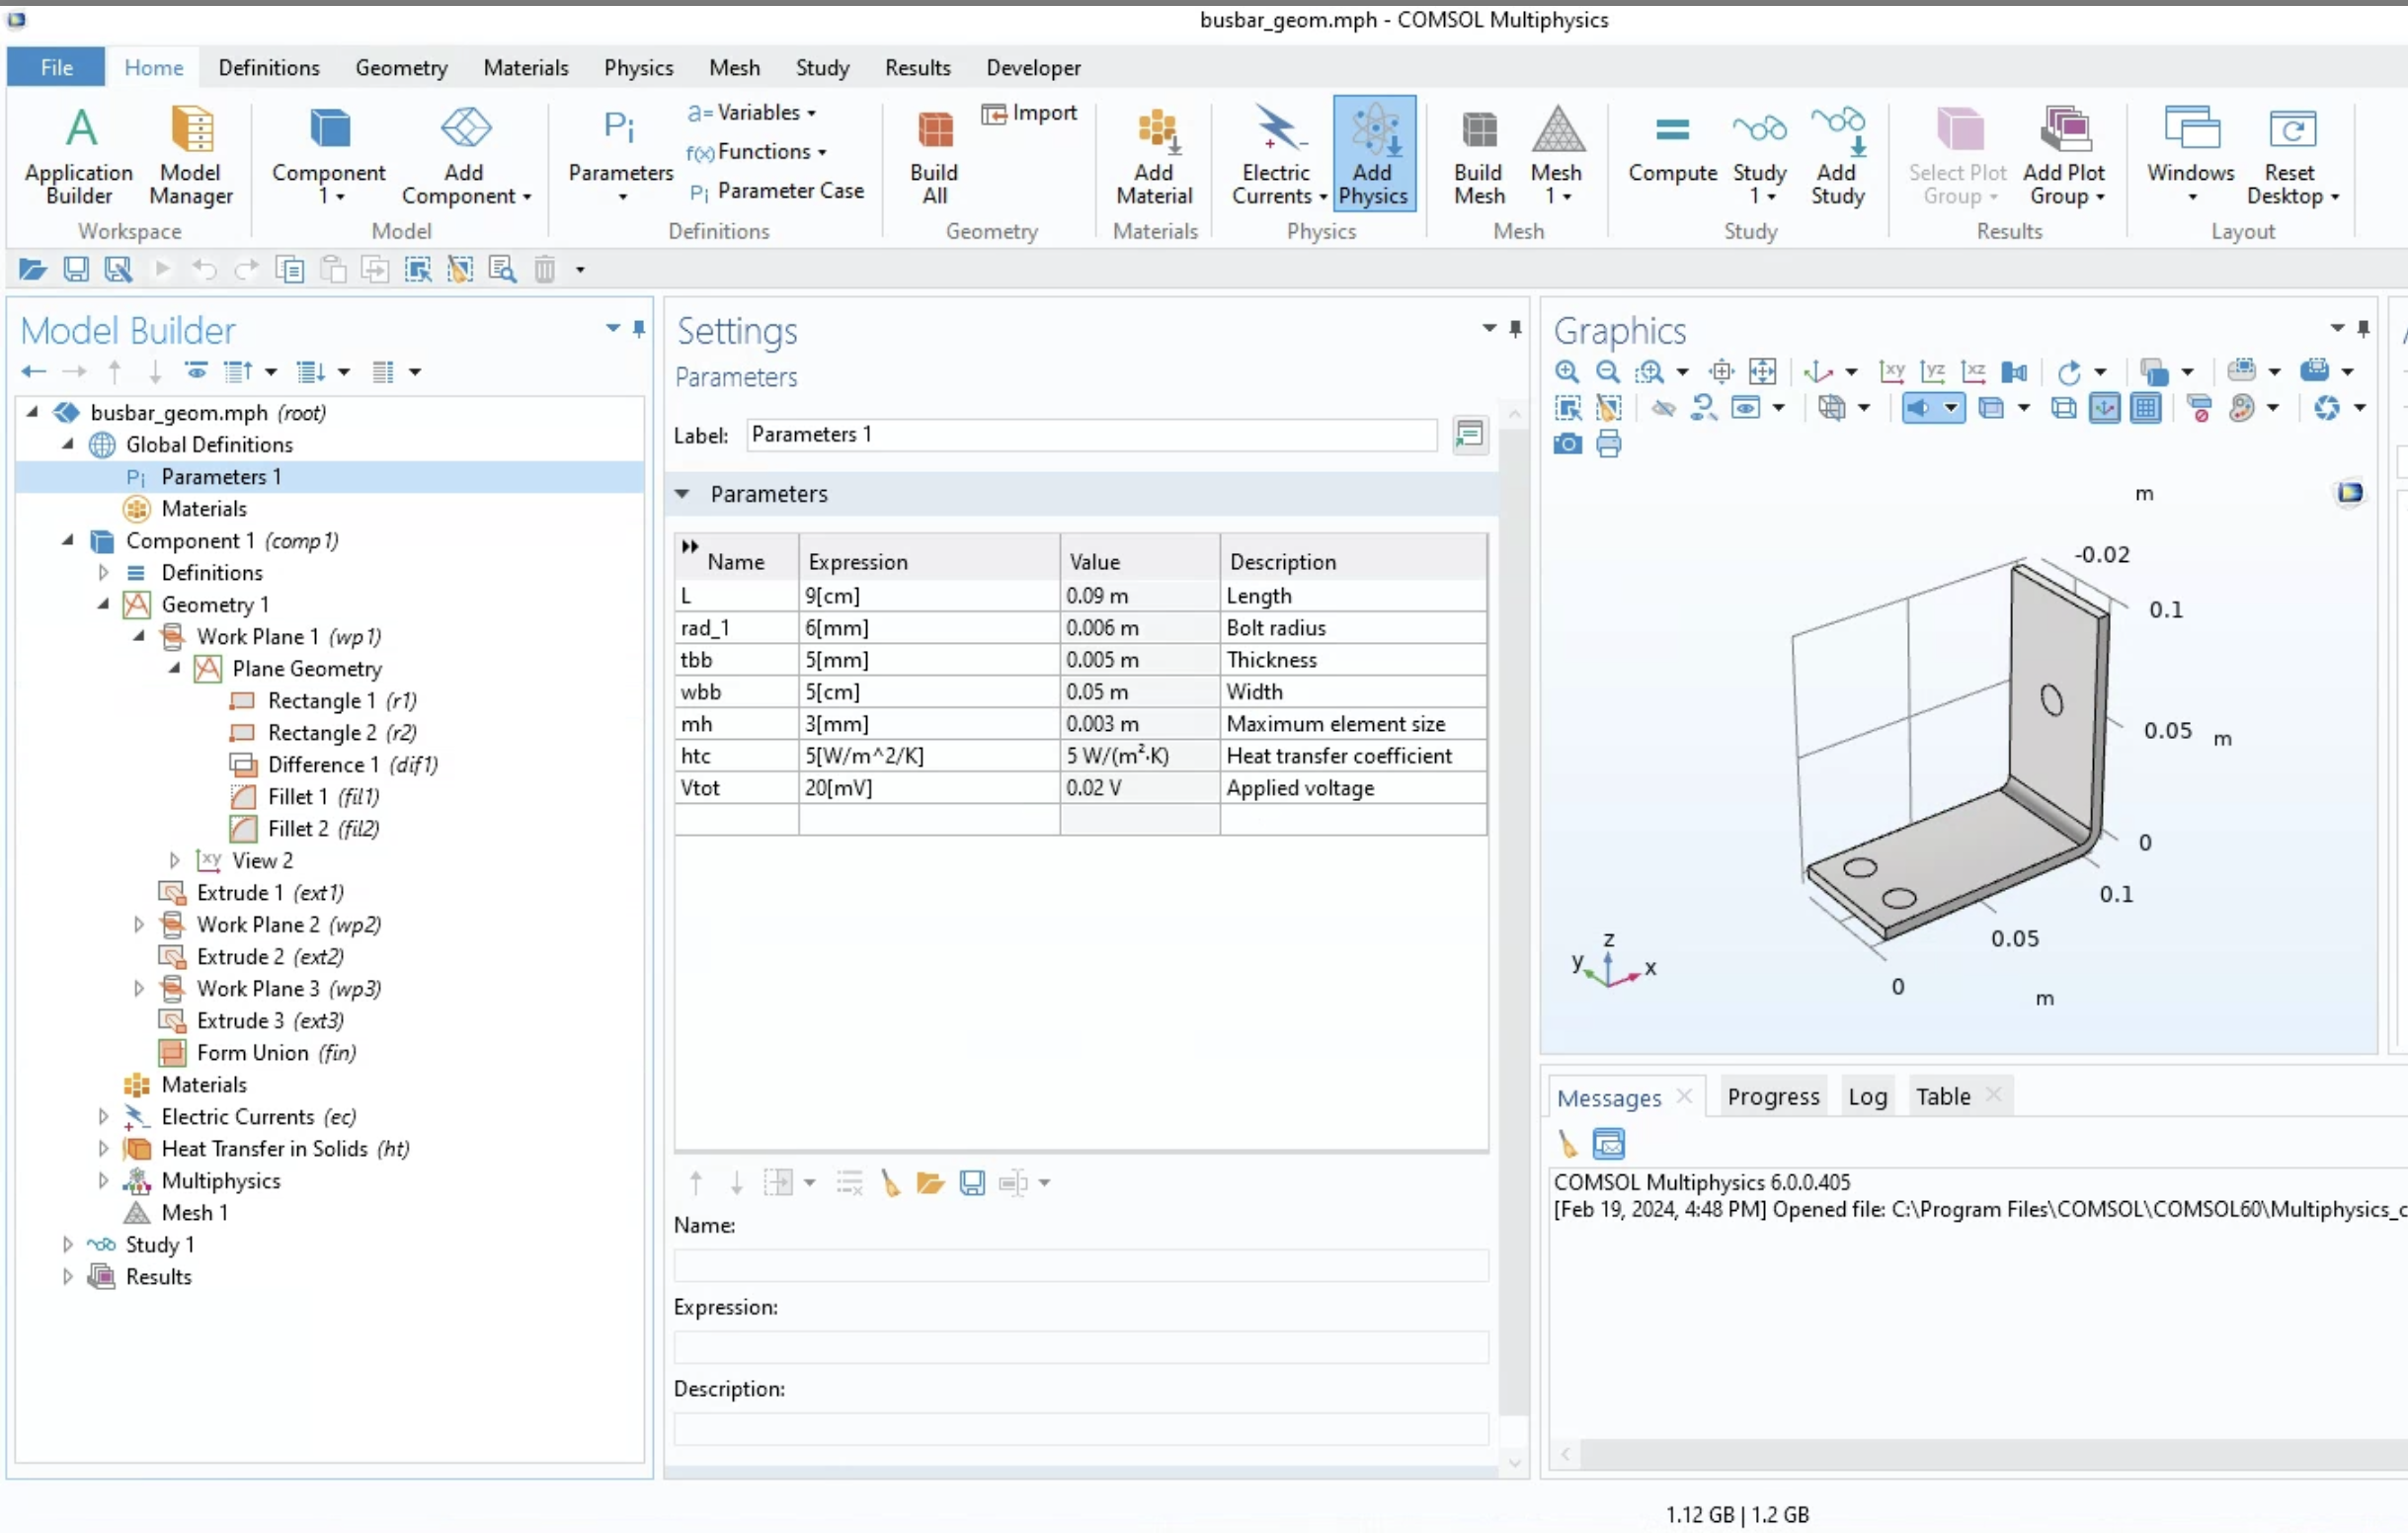
\includegraphics[width=0.7\textwidth]{Chapters/Figures/Chapter 3 Figures/Initial Busbar Geom.png}
  \caption{COMSOL desktop after adding the busbar geometry. Source: \cite{multiphysics__modeling_nodate}}
  \label{fig:COMSOL desktop after busbar geometry}
\end{figure}

% SUBSECTION --- Specifying the Material Properties ---
\subsection{Specifying the Material Properties}.

Our busbar comprises various components each requiring distinct materials, necessitating batch assignment of materials to selected parts rather than individual allocation. To commence, access the Definitions tab and opt for the Explicit selection.

% TODO: Add explicit choice selection from Definitions tab
\begin{figure}[H]
  \centering
  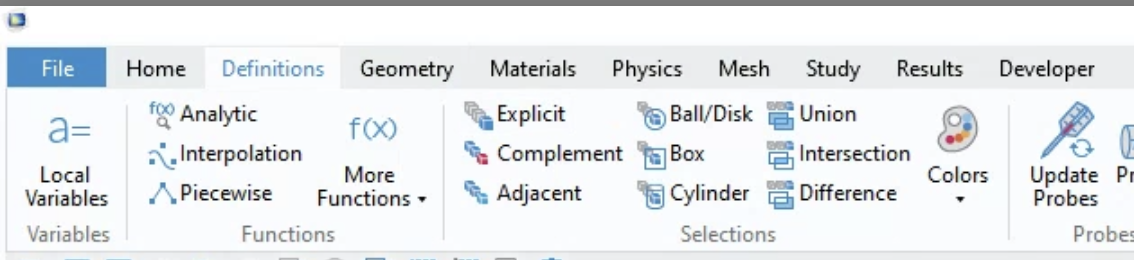
\includegraphics[width=0.7\textwidth]{Chapters/Figures/Chapter 3 Figures/Explicit Choice Selection from Definitions Tab.png}
  \caption{Explicit choice from the Definitions tab. Source: \cite{multiphysics__modeling_nodate}}
  \label{fig:Explicit choice from the Definitions tab.}
\end{figure}

Following this, in the Graphics window, I identify and select the bolts, ensuring both their front and back sides are chosen due to their differing material composition from the busbar's main body.

% TODO: Add bolt selections after selections
\begin{figure}[H]
  \centering
  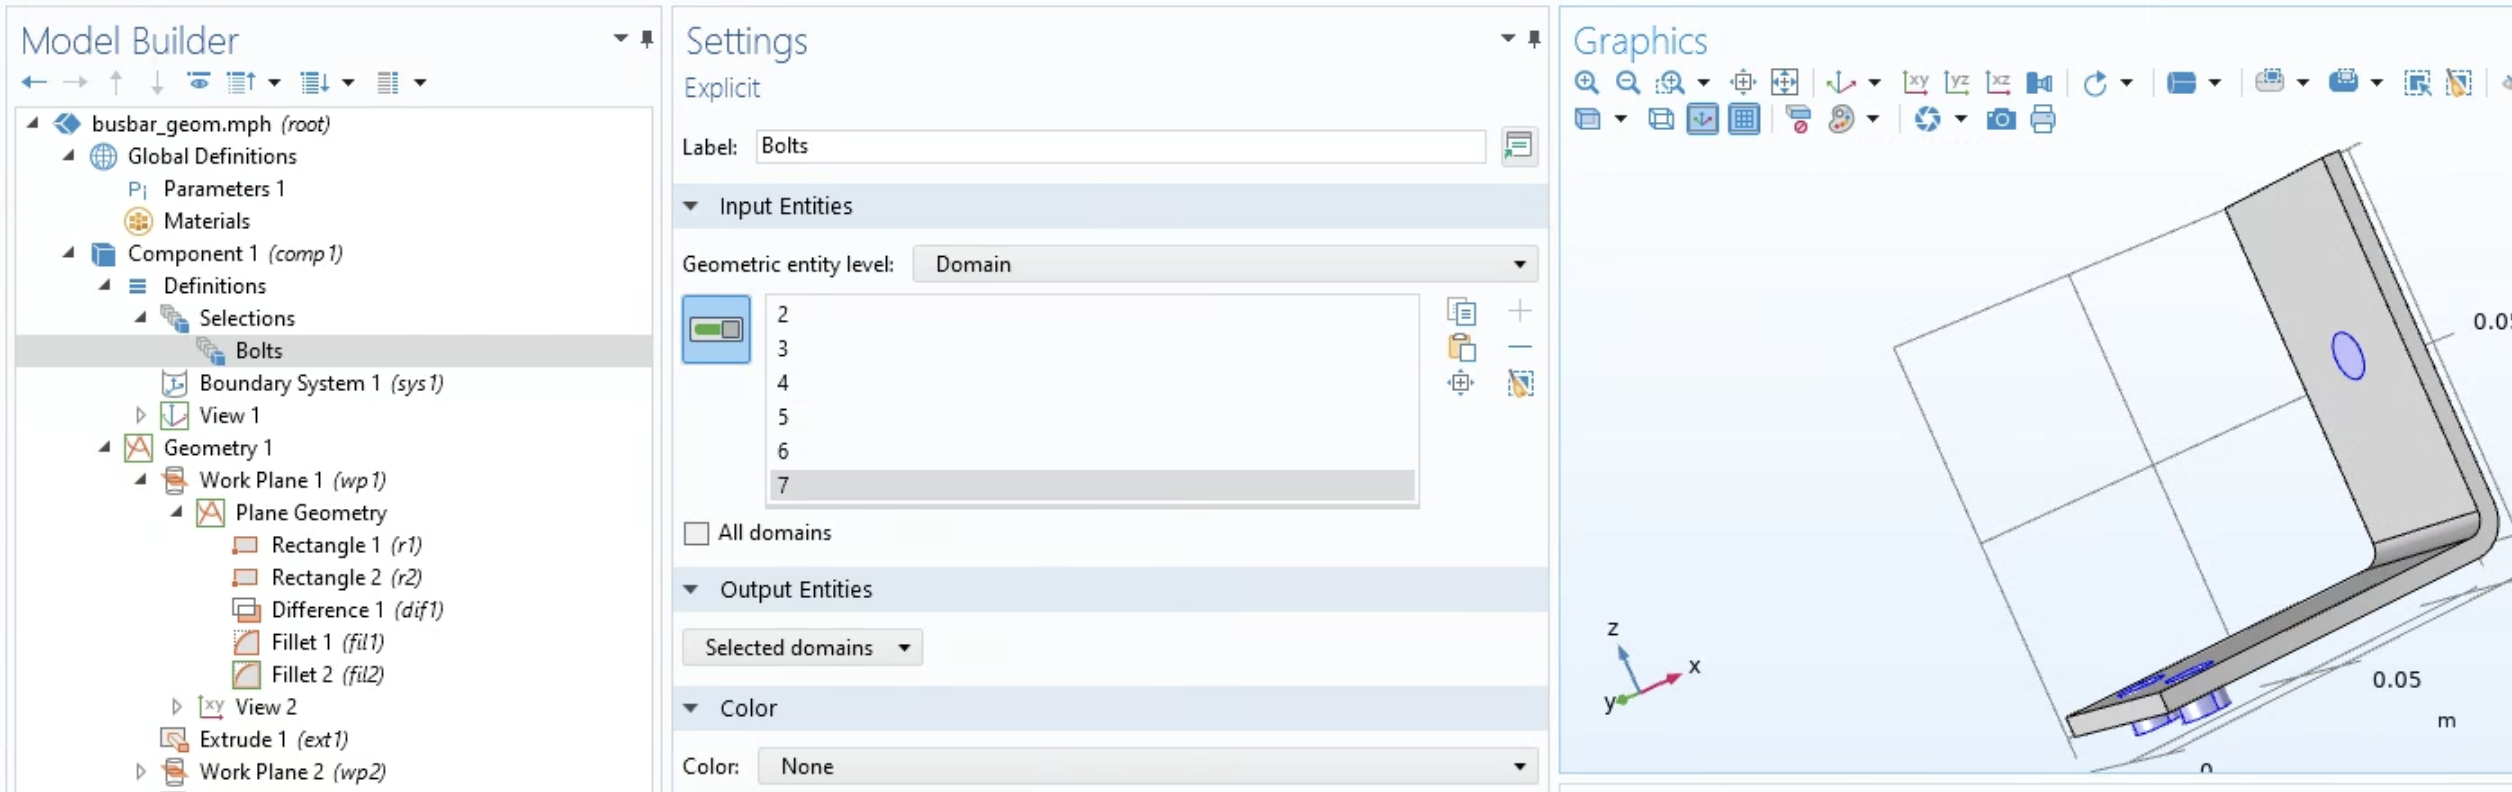
\includegraphics[width=0.7\textwidth]{Chapters/Figures/Chapter 3 Figures/Bolts Selection.png}
  \caption{Adding bolt selections. Source: \cite{multiphysics__modeling_nodate}}
  \label{fig:Adding bolt selections}
\end{figure}

Proceeding to material assignment, I move to the Materials ribbon and select the Add Materials feature. This action opens the ``Add Material'' window, offering a selection of materials to apply to the chosen components.

% TODO: Add the Add Materials image
\begin{figure}[H]
  \centering
  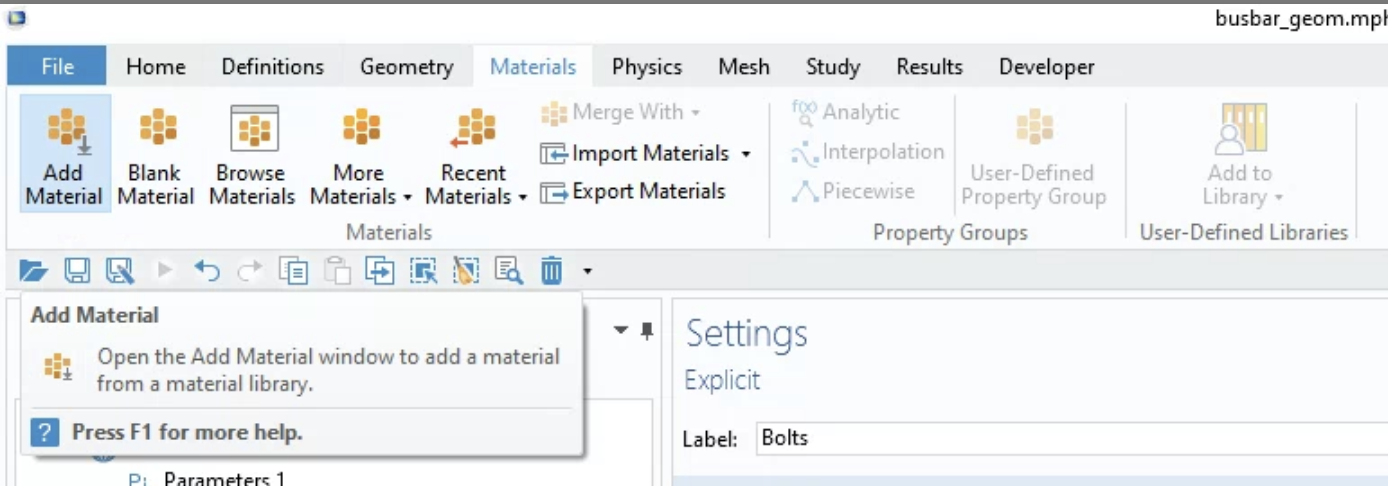
\includegraphics[width=0.7\textwidth]{Chapters/Figures/Chapter 3 Figures/Add Material Button.png}
  \caption{Add Materials option from Materials tab. Source: \cite{multiphysics__modeling_nodate}}
  \label{fig:Add Materials option from Materials tab.}
\end{figure}

Select the Built-In option and opt for Titanium (for the bolts) and Copper as the materials.

% TODO: Add the Add Materials window image
\begin{figure}[H]
  \centering
  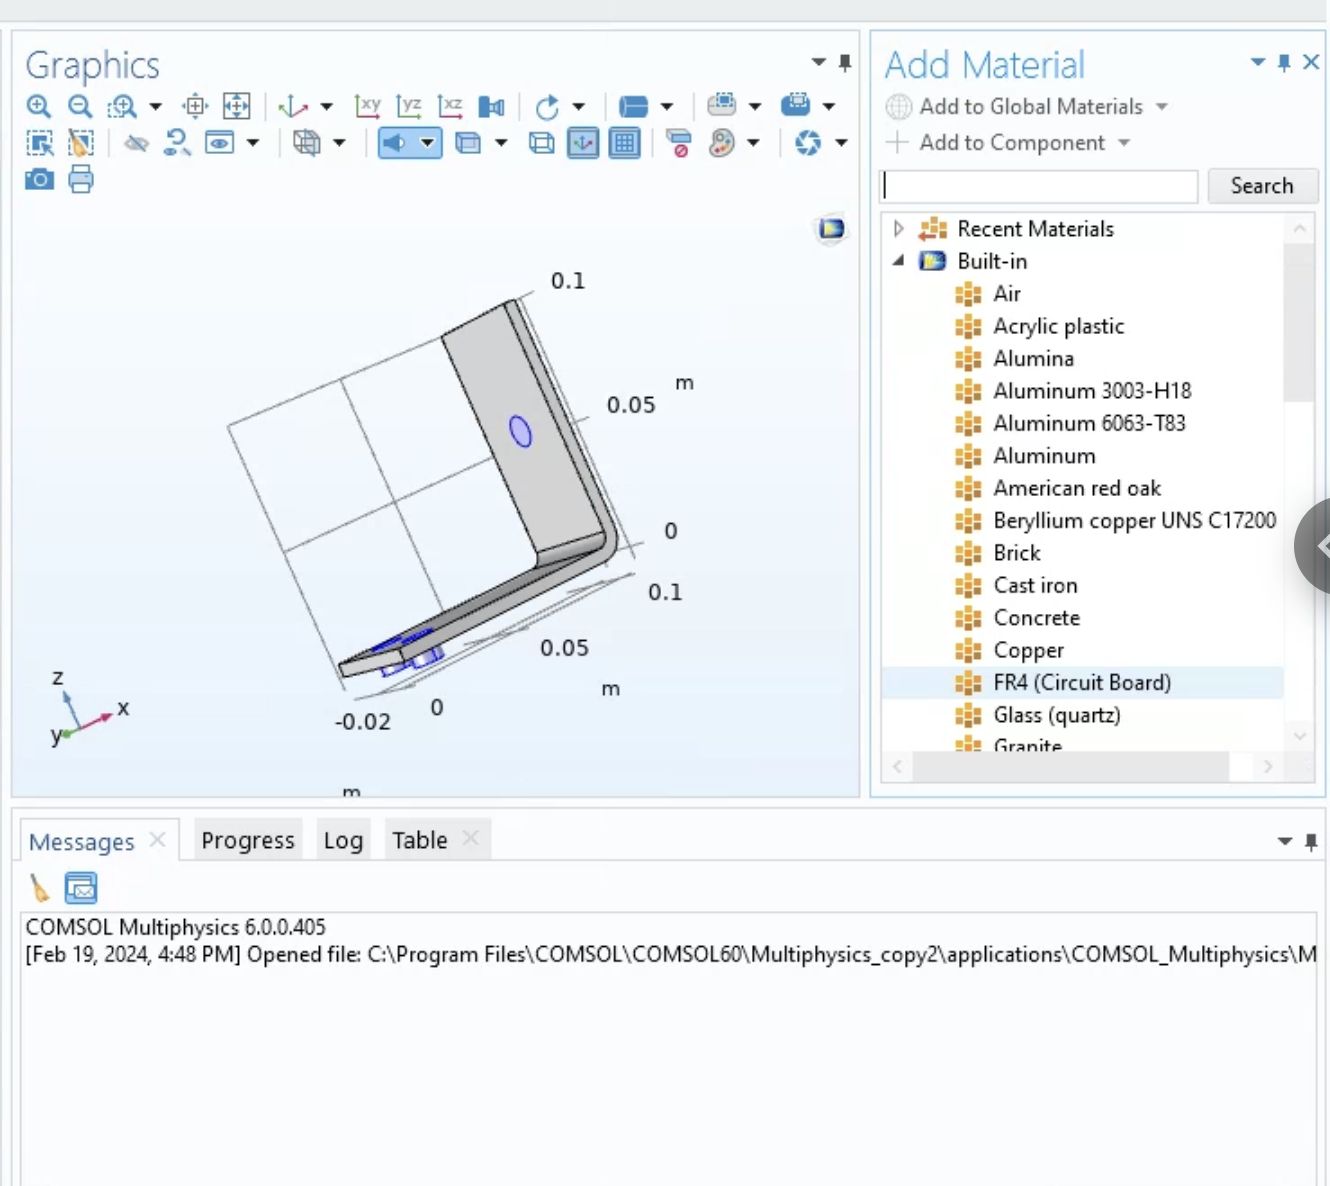
\includegraphics[width=0.7\textwidth]{Chapters/Figures/Chapter 3 Figures/Add Material Window.png}
  \caption{Add Materials window. Source: \cite{multiphysics__modeling_nodate}}
  \label{fig:Add Materials window.}
\end{figure}

The earlier defined selection for Bolts proves useful now as I assign Titanium to each bolt by selecting the Bolts option, as illustrated below.

% TODO: Add the bolts for titanium material selection
\begin{figure}[H]
  \centering
  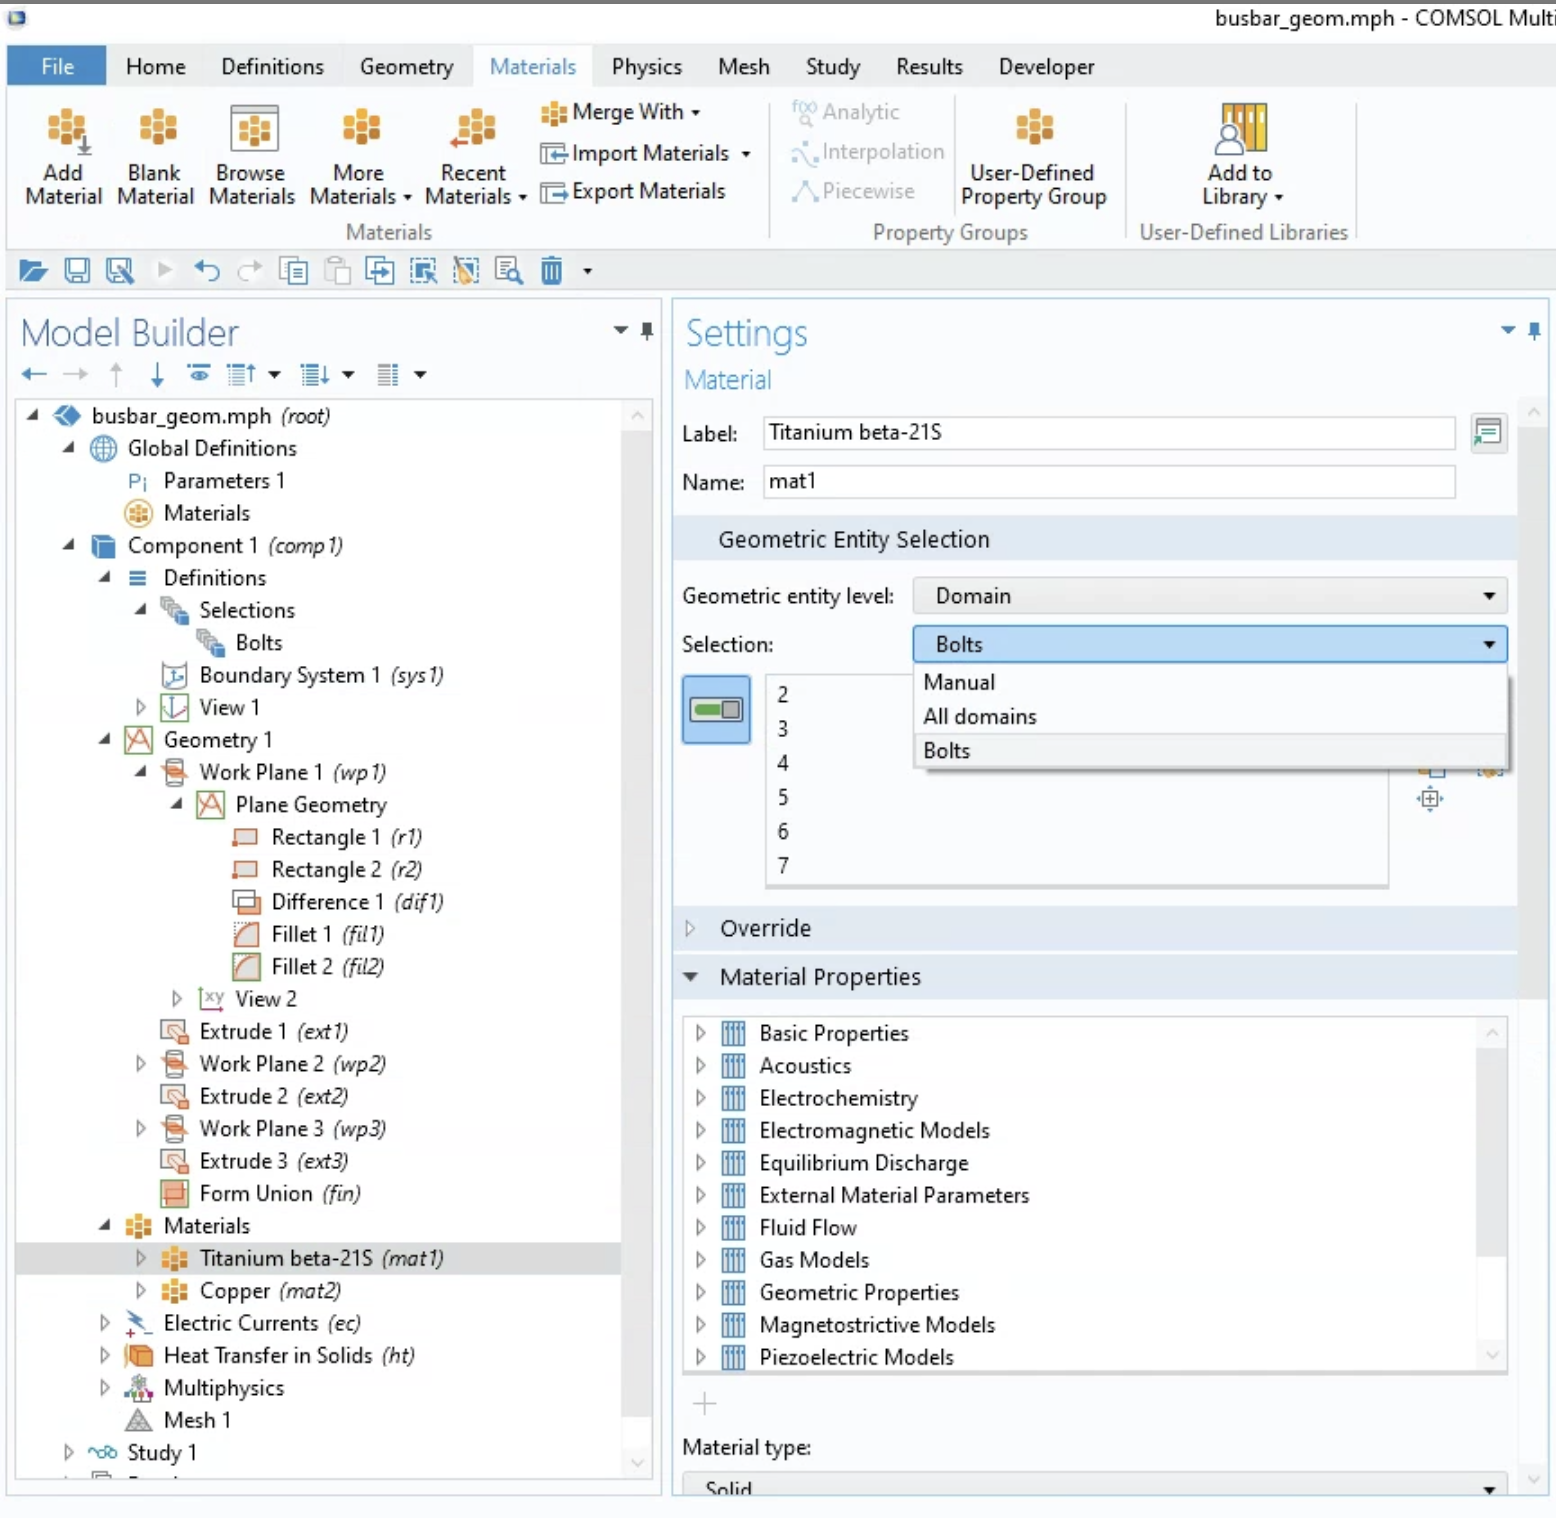
\includegraphics[width=0.7\textwidth]{Chapters/Figures/Chapter 3 Figures/Bolts Selection Choice.png}
  \caption{Assigning some bolts to be made of Titanium. Source: \cite{multiphysics__modeling_nodate}}
  \label{fig:Assigning some bolts to be made of Titanium.}
\end{figure}

Every time a material is added, and consequently a material node is introduced in the Model Builder window, a table appears in the Settings window under Material Contents. This table details the physical properties of the respective materials, including Electrical Conductivity, Heat Capacity, and more.

% TODO: Add image showing material contents (properties)
\begin{figure}[H]
  \centering
  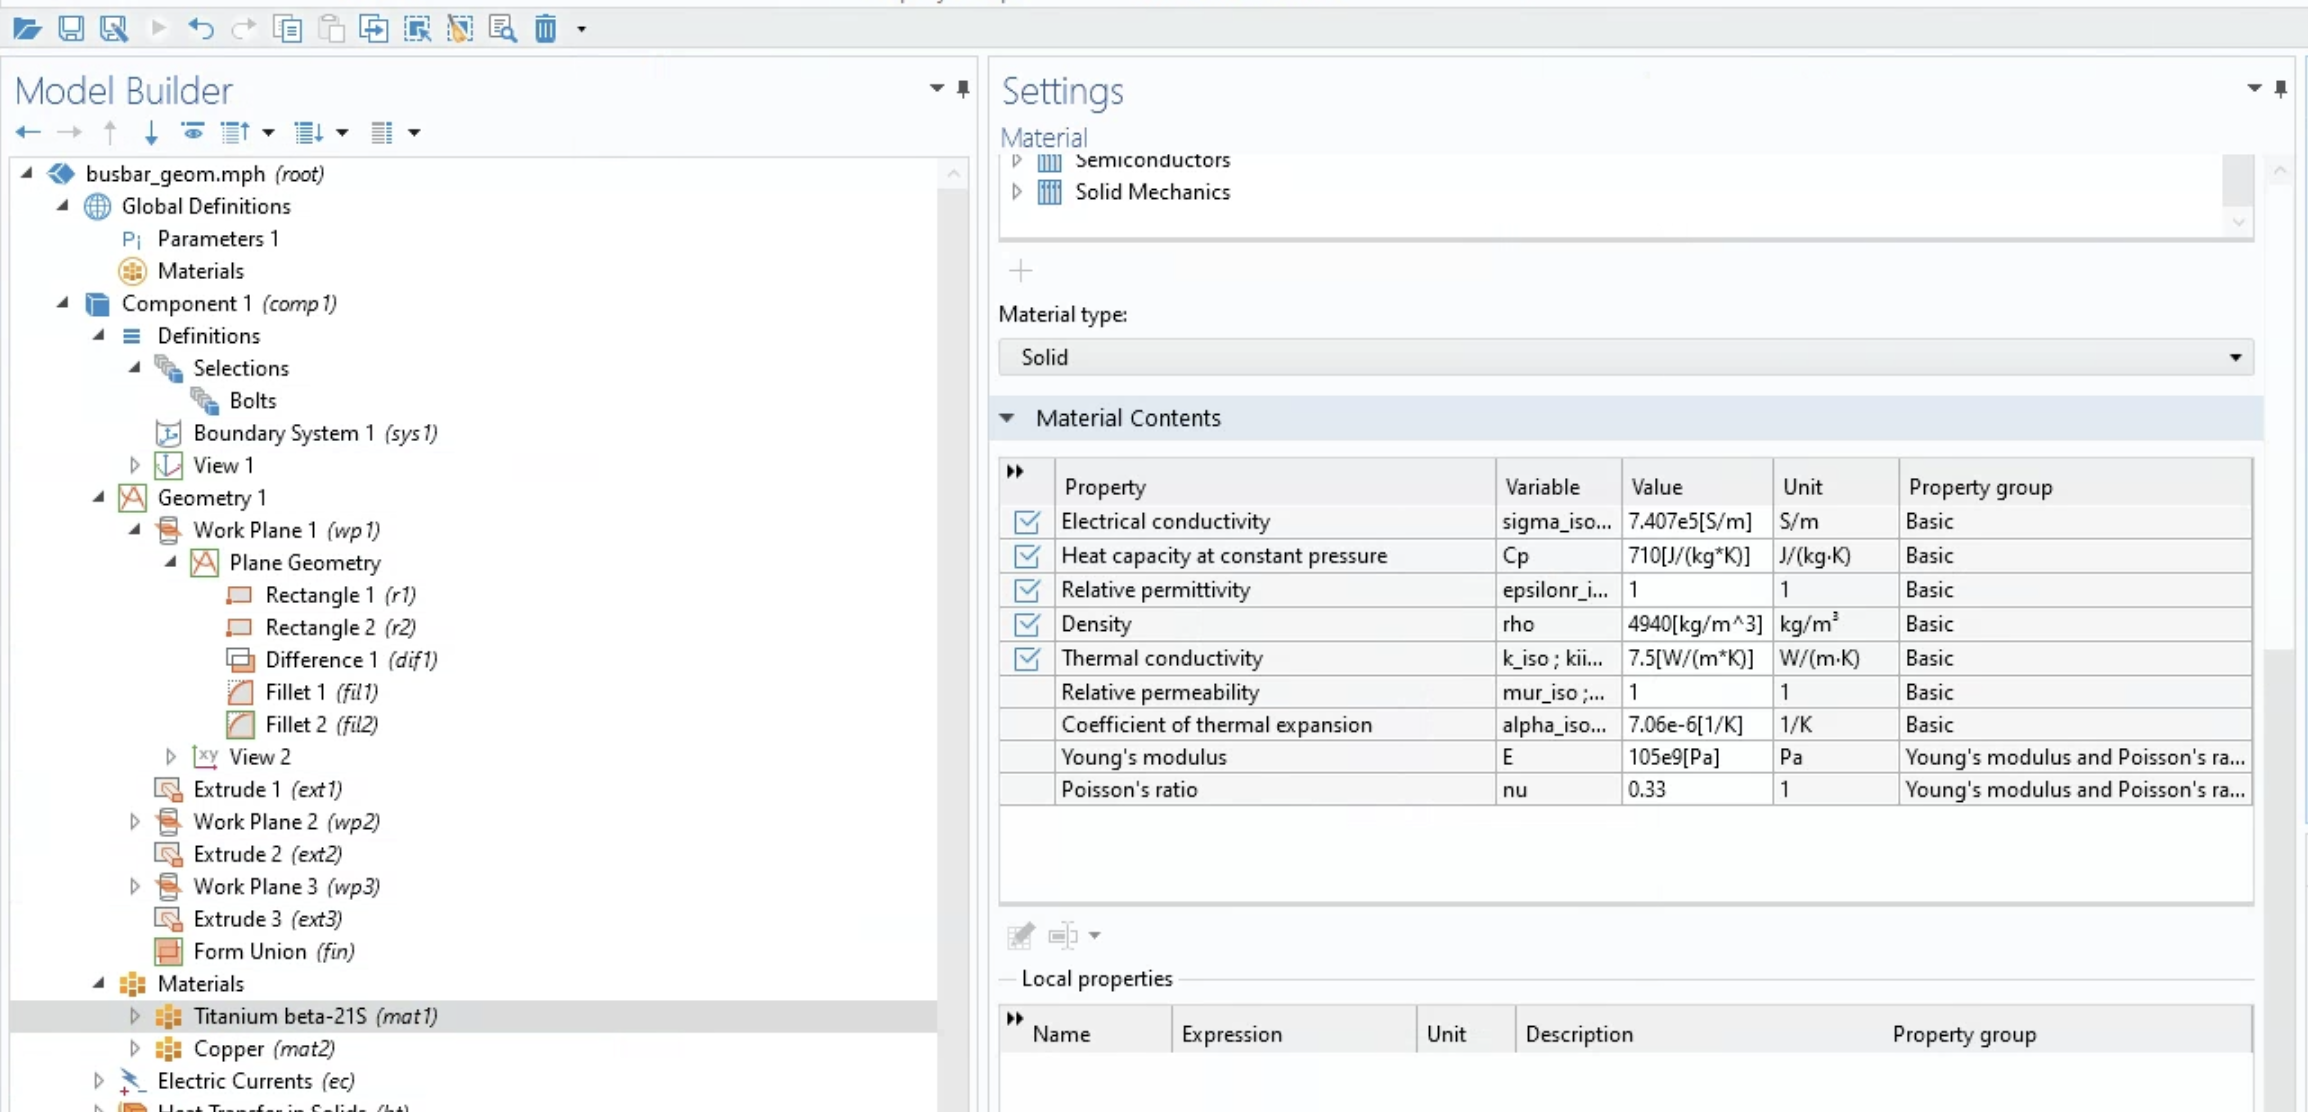
\includegraphics[width=0.7\textwidth]{Chapters/Figures/Chapter 3 Figures/Material Contents in Settings Window.png}
  \caption{Material Properties. Source: \cite{multiphysics__modeling_nodate}}
  \label{fig: Material properties.}
\end{figure}

% SUBSECTION --- Defining the Physics Boundary Conditions ---
\subsection{Defining the Physics Boundary Conditions}
It is time to apply mathematical formulas across various sections of our model to replicate the intended physics. This involves highlighting specific segments of the geometry and imposing relevant formulas and physical parameters that accurately represent those segments.

I will begin by setting up the physics for the electric current interface, aiming to model the flow of electricity from a singular bolt across to the twin bolts at the opposite end of the busbar. The specific physics chosen during the initial model setup might already have certain equations predefined within their physics nodes. For example, within the ``Electric Currents (ec)'' node, the settings window reveals equations pertinent to this physics. A key equation presented is the fundamental one linking the electric field with electric potential, expressed as $\mathbf{E} = -\nabla V$.

% TODO: Add image showing equation
\begin{figure}[H]
  \centering
  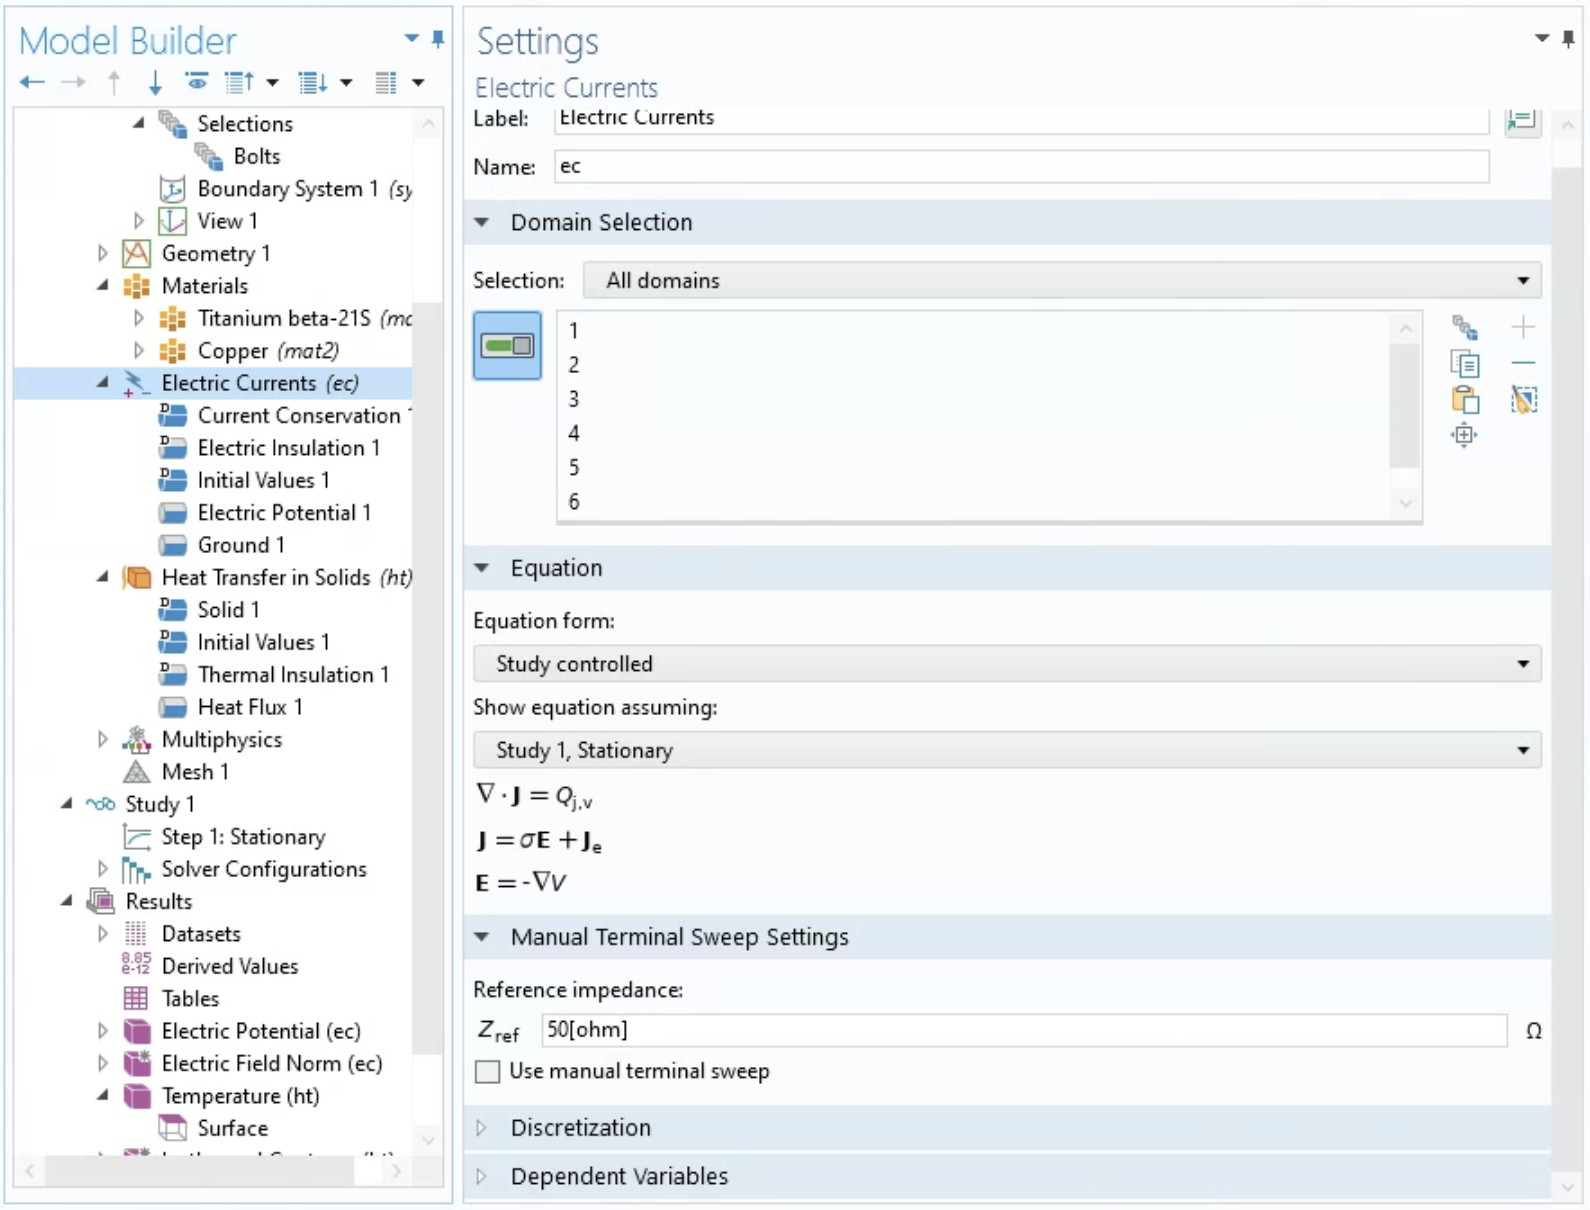
\includegraphics[width=0.7\textwidth]{Chapters/Figures/Chapter 3 Figures/Electrical Currents Physics Equation.png}
  \caption{The corresponding guiding equation. Source: \cite{multiphysics__modeling_nodate}}
  \label{fig:the guiding equation}
\end{figure}

COMSOL Multiphysics operates transparently, allowing users to fully grasp the software's actions and methodologies.

Upon integrating physics into our model, several default nodes were automatically established within each physics category. I add specific boundary conditions and constraints only if they deviate from these defaults. For example, the ``Electric Currents (ec)'' physics automatically applies the ``Electric Insulation 1'' condition to all boundaries, which may not suit our model's requirements.

For our purpose, I aim to impose a voltage on the bottom surface of the single bolt. This is achieved by navigating to the Physics tab, selecting Boundaries, and then choosing Electric Potential. This action adds an ``Electric Potential 1'' node. The next step is to identify and select the geometry segment this potential will affect. To specify the electric potential value, I input 20 mV, denoted as 20[mV], with the brackets indicating unit specification.

To simplify the process, remember that the ``Parameters 1'' node contains a predefined variable, Vtot, representing the applied voltage. Utilizing this variable instead of inputting 20[mV] directly facilitates the setup of parametric studies in the future.

Finally, to complete our setup, I establish a ground boundary condition on the bottom surfaces of the two bolts at the busbar's opposite end. This is accomplished by selecting Ground from the Physics tab's boundaries options, then choosing the relevant geometry segments.

% TODO: Add image showing "Electric Currents" boundary conditions
\begin{figure}[H]
  \centering
  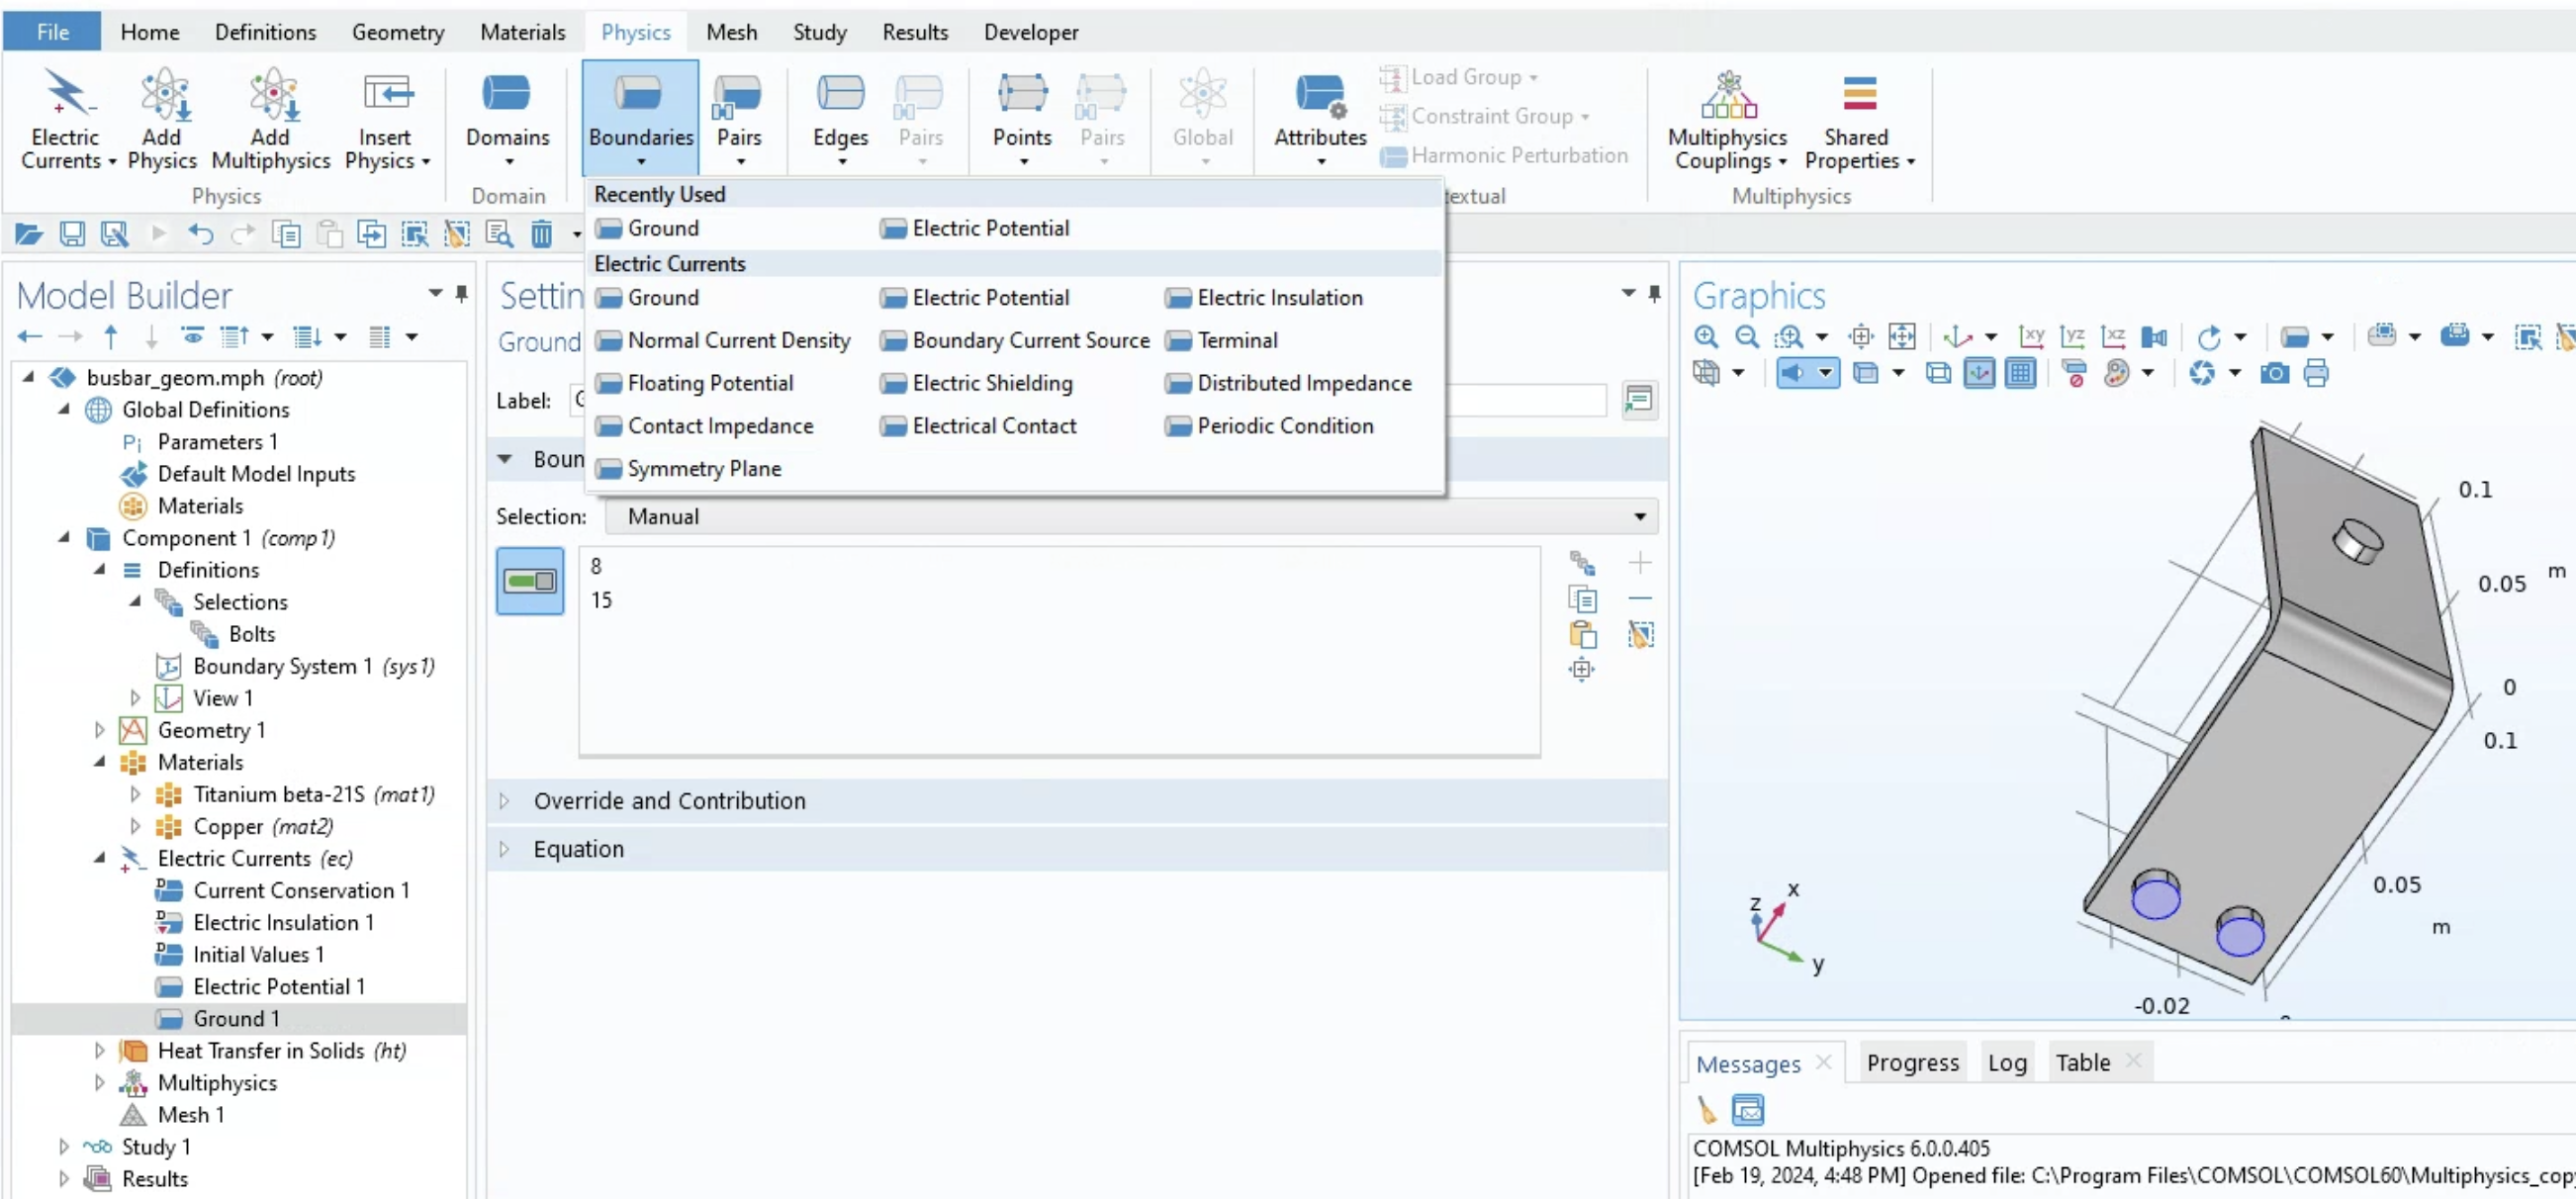
\includegraphics[width=0.7\textwidth]{Chapters/Figures/Chapter 3 Figures/Electric Currents Boundary Conditions.png}
  \caption{Electric Currents boundary conditions. Source: \cite{multiphysics__modeling_nodate}}
  \label{fig:Electric Currents boundary conditions}
\end{figure}

Given the selection of Joule Heating as a coupled physics in our model, it is essential to define the thermal boundary conditions as well. The default ``Thermal Insulation 1'' condition, which applies universally across our model, does not suit our specific needs. To address this, proceed to the Physics tab, access Boundaries, and opt for Heat Flux. Within the settings, under Boundary Selection, choose ``All Boundaries'' but exclude the previously selected bolt surfaces for the Electric Currents boundaries—namely, boundaries 8, 15, and 43—by deselecting these numbers using the ``Remove from Selection'' option.

For the Heat Flux settings, opt for the ``Convective heat flux'' under the Flux Type category, entering a value of 5 $W/(m^2\cdot K)$. Similar to our approach with the electric potential, revert to the Parameters 1 node and input $htc$, which denotes the value of 5 $W/(m^2\cdot K)$.

% TODO: Add image showing Heat Flux boundary conditions
\begin{figure}[H]
  \centering
  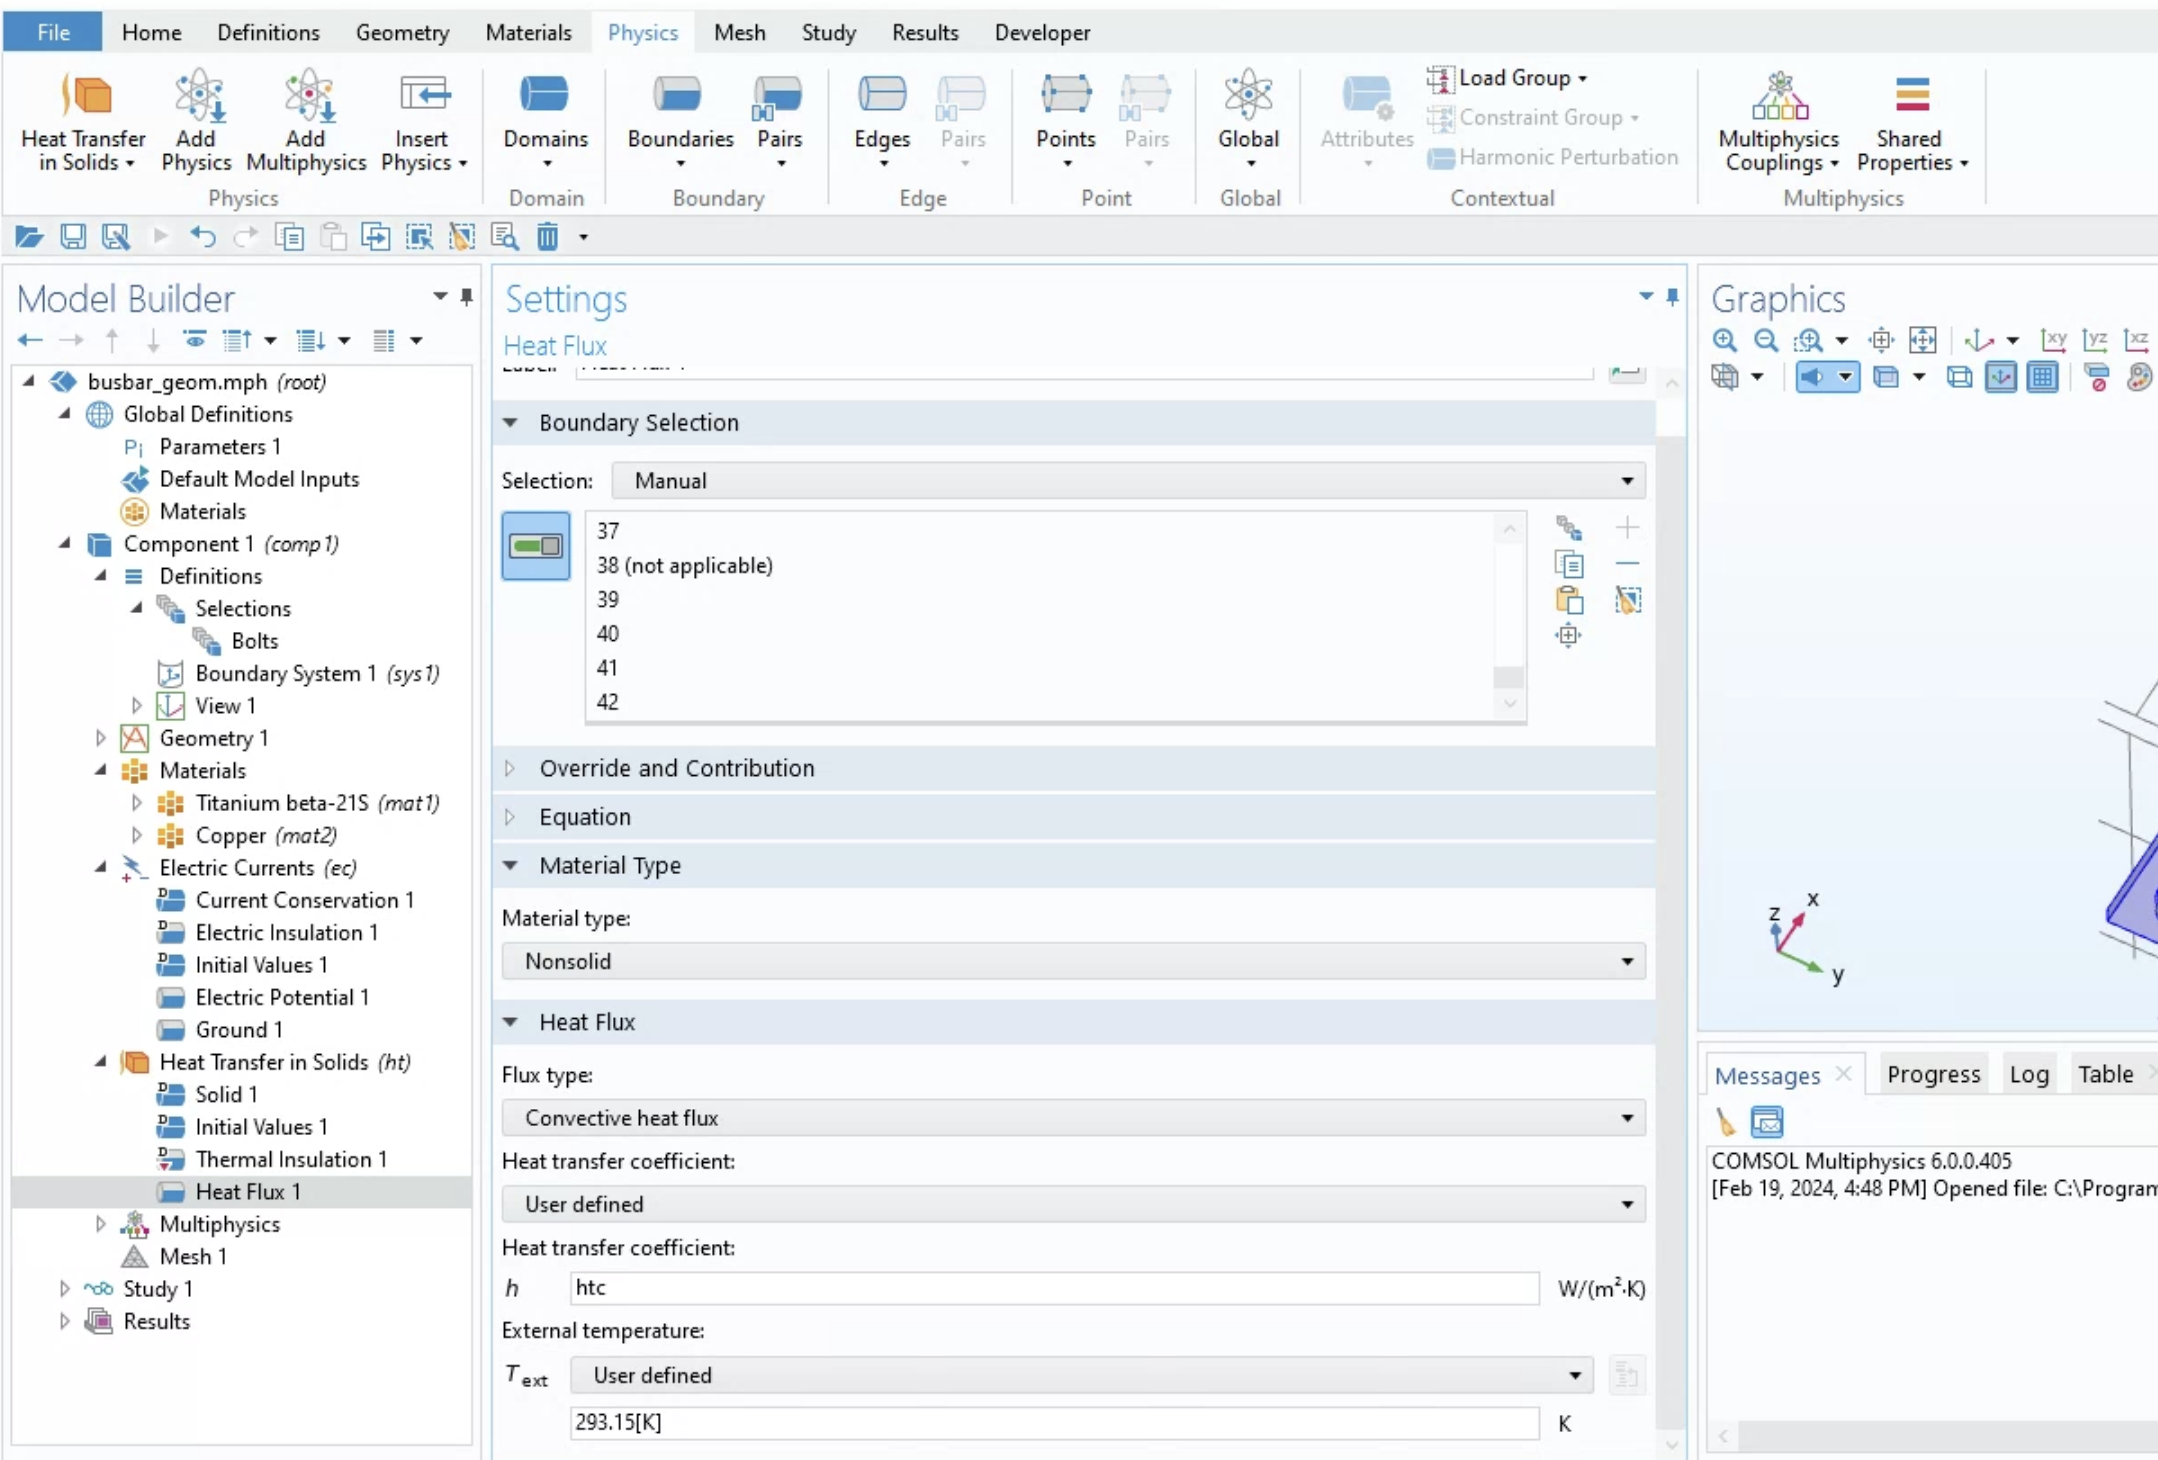
\includegraphics[width=0.7\textwidth]{Chapters/Figures/Chapter 3 Figures/Heat Flux Boundary Conditions.png}
  \caption{Heat Flux boundary conditions. Source: \cite{multiphysics__modeling_nodate}}
  \label{fig:Heat Flux boundary conditions.}
\end{figure}

In our busbar model, the two physics components I have incorporated, namely Electric Currents and Heat Transfer in solids, are universally applicable throughout the model.

% SUBSECTION --- Build the Mesh ---
\subsection{Build the Mesh}
Navigate to the Mesh ribbon and initiate mesh configuration by selecting ``Mesh 1.'' Within the Settings, under Mesh Setting, accessing the Sequence Type menu presents two alternatives: the default Physics-controlled mesh, which automatically tailors the mesh to the model's physics requirements, and the user-controlled mesh, granting manual oversight over mesh granularity and enabling the use of diverse element types.

COMSOL Multiphysics accommodates a variety of 2D and 3D element shapes, including pyramids, triangles, and prisms. The software offers nine predefined element size settings, ranging from extremely fine to extremely coarse. To construct the mesh, simply press the ``Build All'' button.

% TODO: Add image showing the mesh of the busbar under "fine"
\begin{figure}[H]
  \centering
  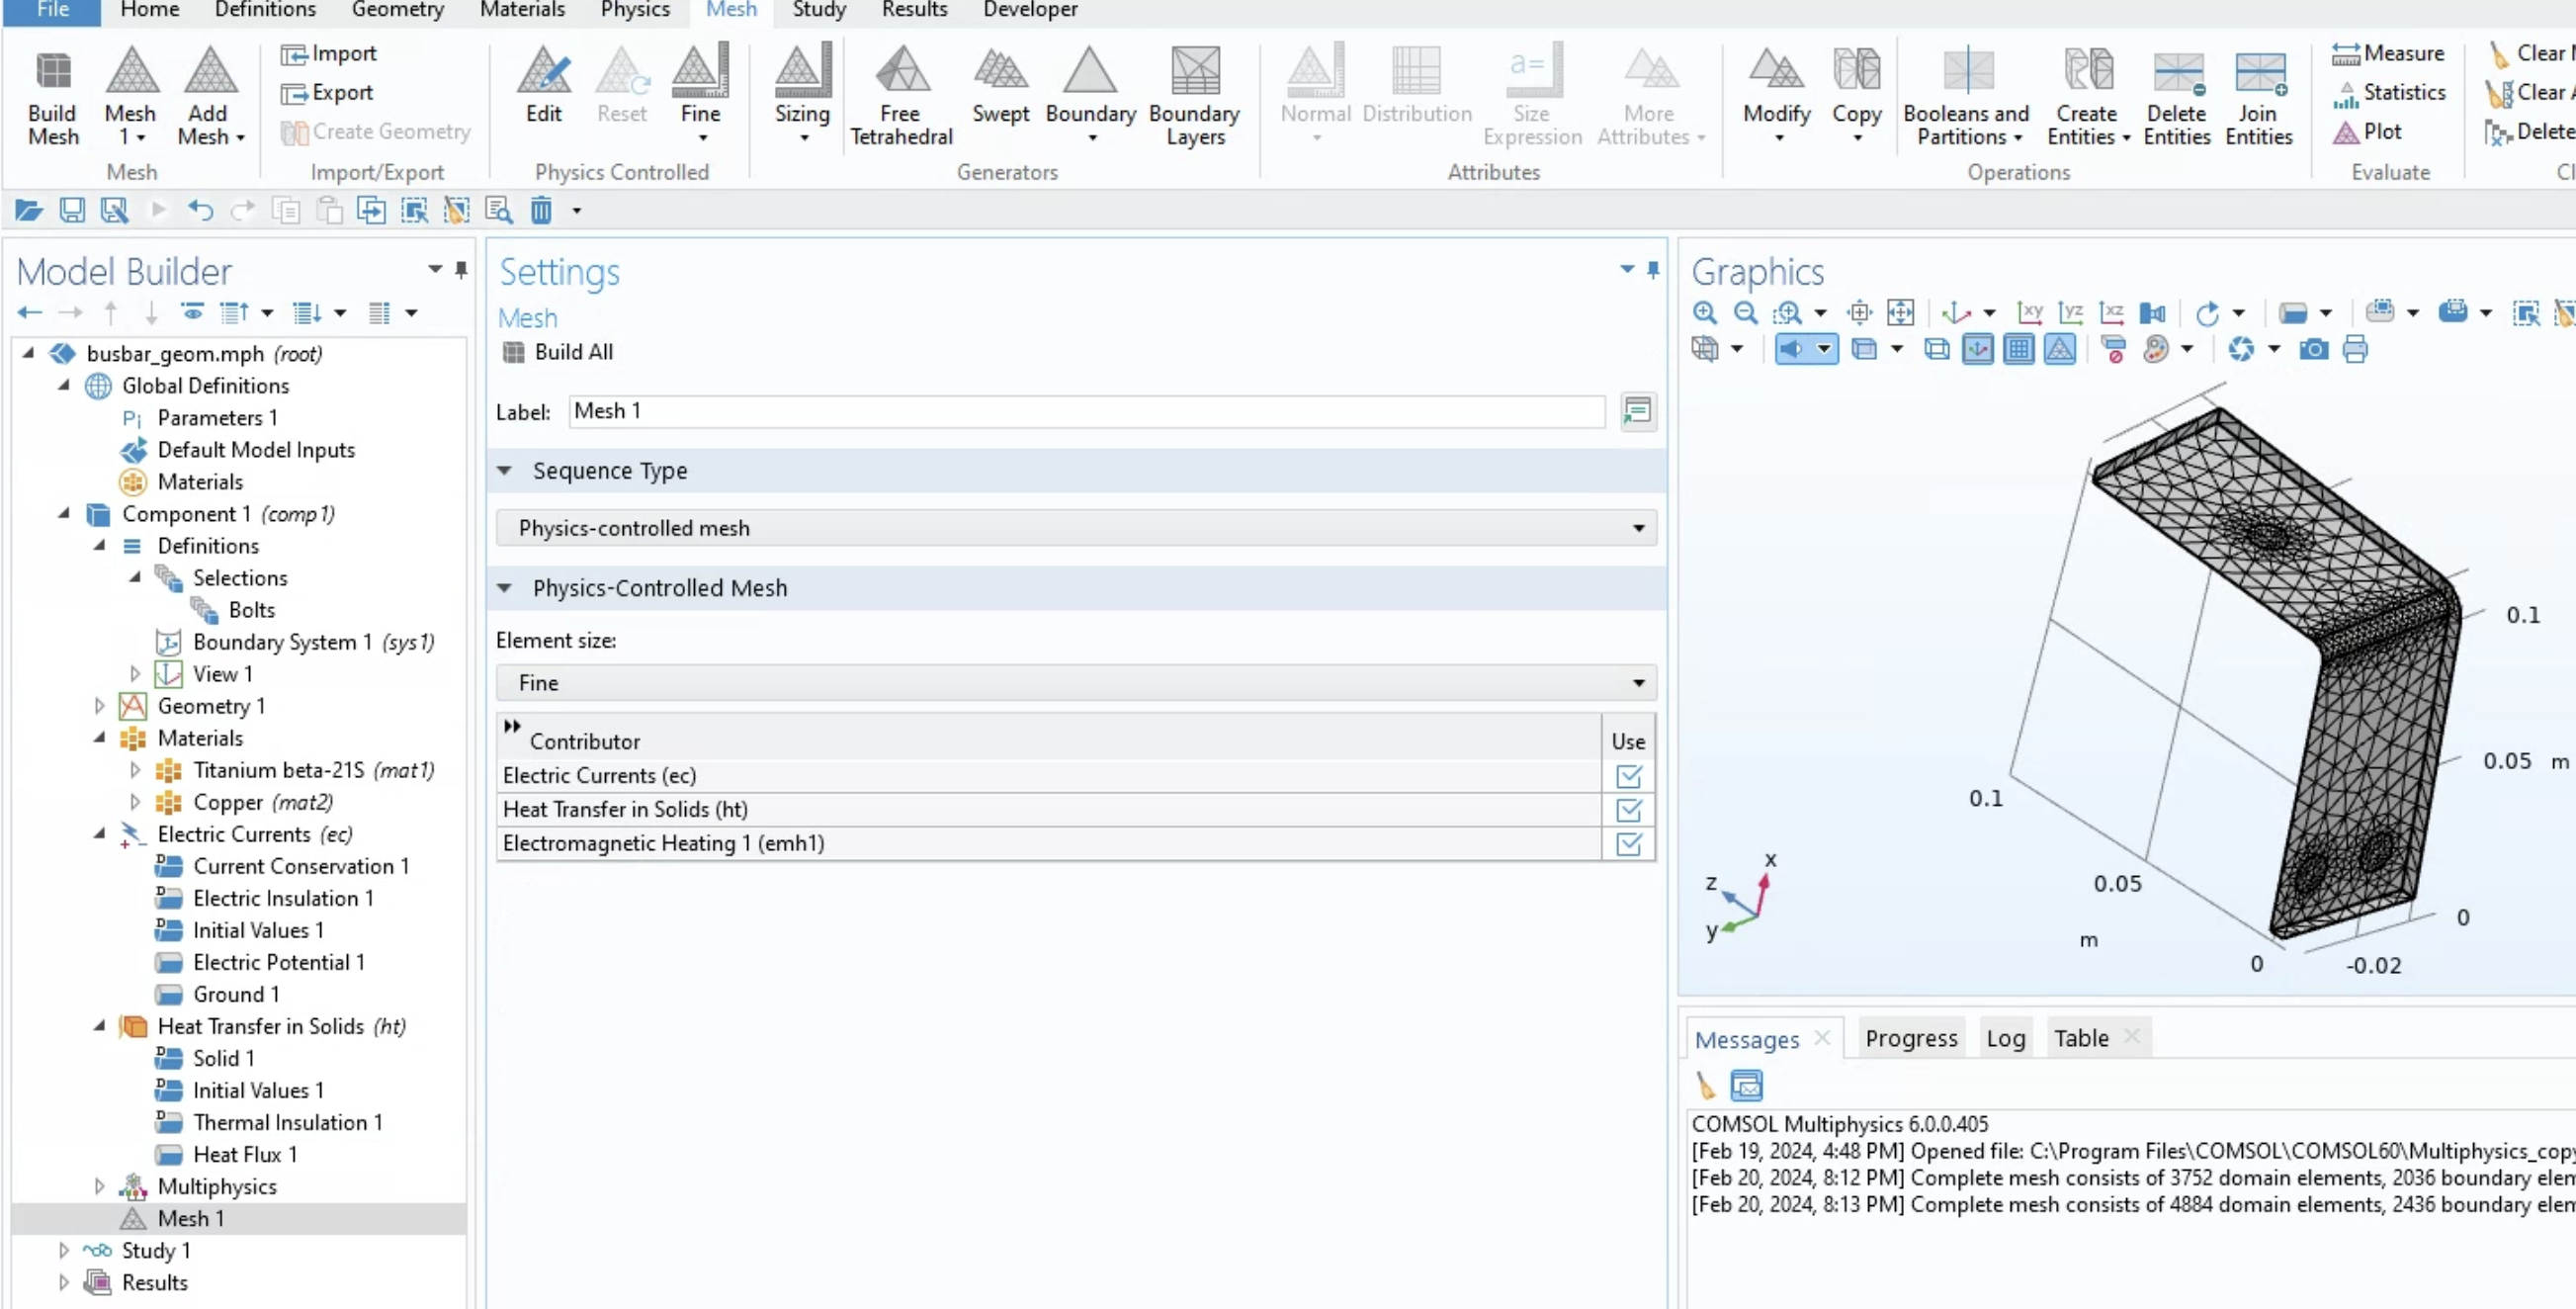
\includegraphics[width=0.7\textwidth]{Chapters/Figures/Chapter 3 Figures/Fine Mesh.png}
  \caption{Fine mesh type. Source: \cite{multiphysics__modeling_nodate}}
  \label{fig:Fine mesh type.}
\end{figure}

% SUBSECTION --- Run the Study ---
\subsection{Run the Study}
By selecting and expanding the ``Study 1'' node within the Settings, there's an option to ``Generate default plots'', which automatically creates visual representations tailored to the physics defined in the model. Given our focus on electric currents and heat transfer, this function will produce plots detailing both the electric potential and the temperature distribution within the busbar.

Under the ``Step 1: Stationary'' sub-node, found in the ``Physics and Variables'' drop-down, the integration of the multi-physics problem within the ``Solve For'' section becomes visible. Proceed by clicking the ``Compute'' button to perform the simulation. Once computation is complete, the process advances to the next phase, which involves the post-processing of the generated results.

% TODO: Add image showing computed results.
\begin{figure}[H]
  \centering
  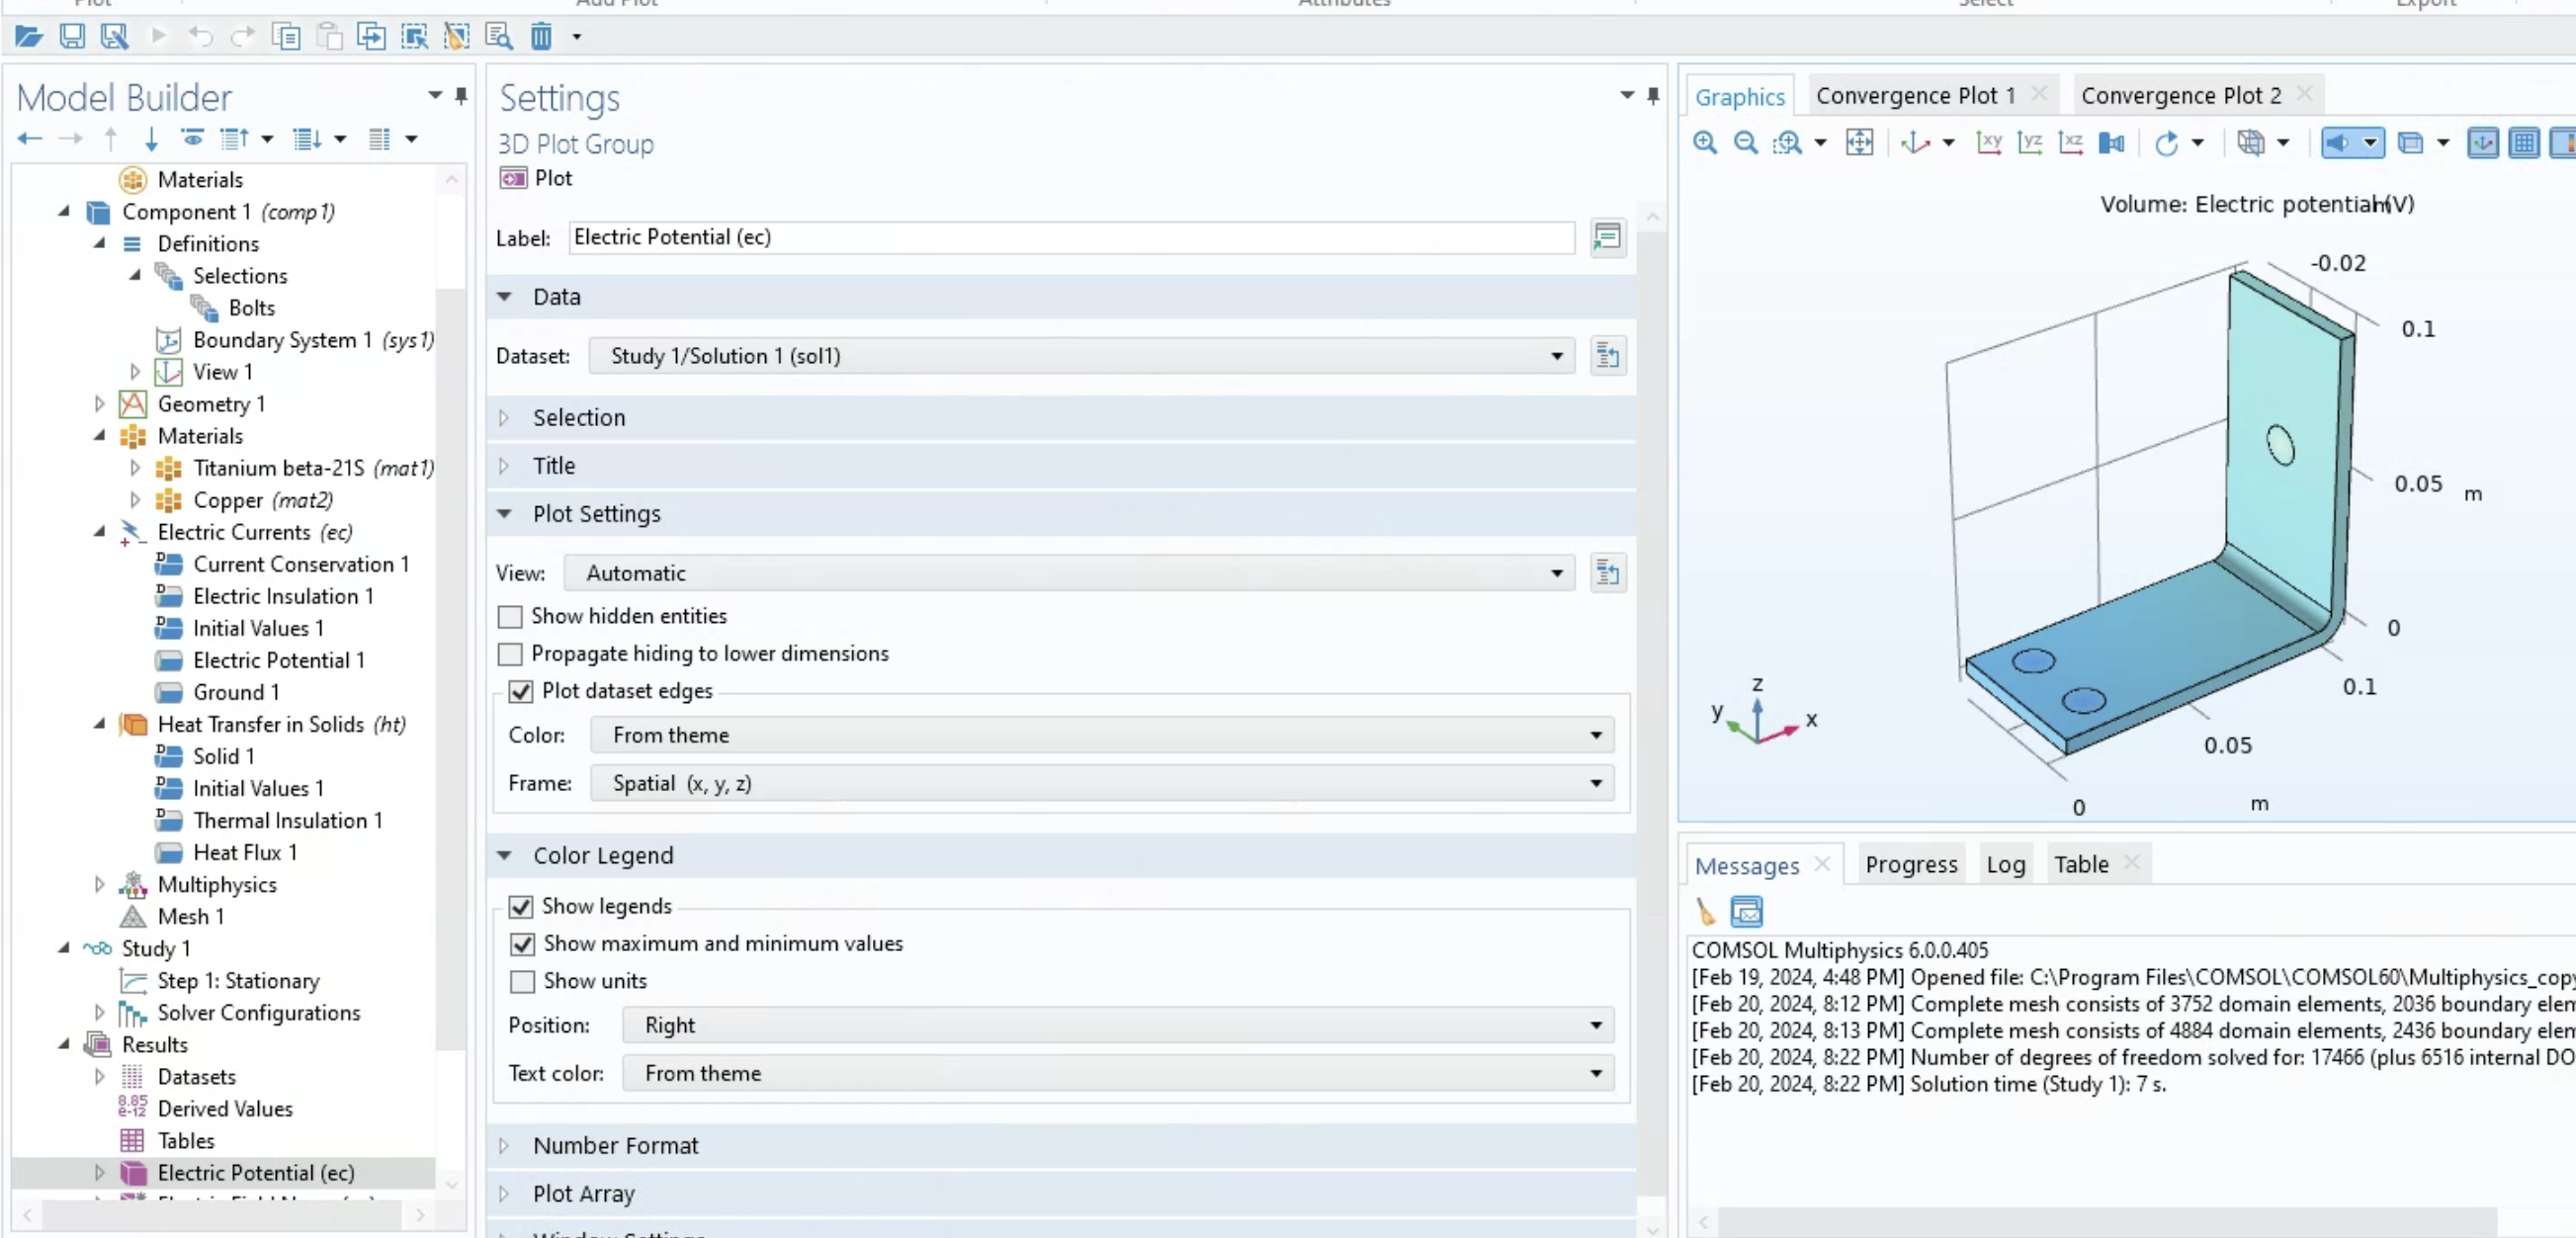
\includegraphics[width=0.7\textwidth]{Chapters/Figures/Chapter 3 Figures/Computed Results.png}
  \caption{Computed results. Source: \cite{multiphysics__modeling_nodate}}
  \label{fig:computed results}
\end{figure}

% SUBSECTION --- Post-Processing the Results ---
\subsection{Post-Processing the Results}
The purpose of post-processing in the model construction process is to convert complex simulation data into a user-friendly format that is accessible and informative. The goal is to create a customisable interface using the Application Builder, which is part of COMSOL Multiphysics software. This interface, or simulation application, enables users, often those without extensive simulation background, to explore the model by varying key parameters and instantly visualizing the effects.

Accessible directly from the home toolbar, the Application Builder is an integral tool for enhancing the interactivity and accessibility of the simulation results. The process begins with transforming the busbar model into an interactive application that allows for the modification of predetermined parameters such as the busbar's length, width, and applied voltage.

\begin{figure}[H]
    \centering
    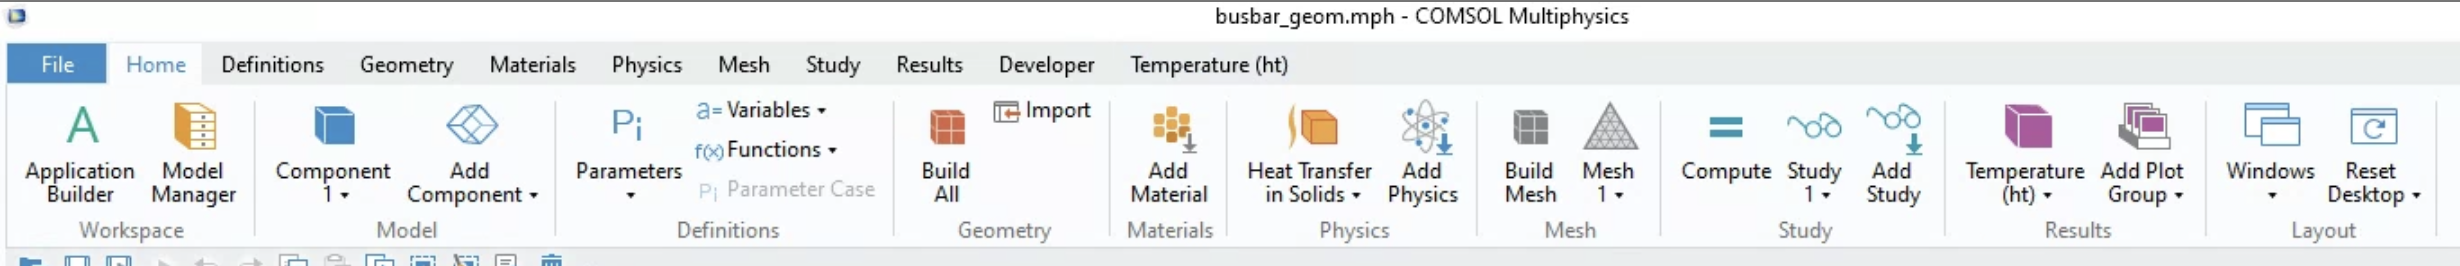
\includegraphics[width=0.7\textwidth]{Chapters/Figures/Chapter 3 Figures/Application Builder Button.png}
    \caption{Application builder button. Source: \cite{multiphysics__modeling_nodate}}
    \label{fig:application builder button}
\end{figure}

To streamline the creation of the application, I utilize the New Form Wizard, a feature designed for rapid app development within the Application Builder.

\begin{figure}[H]
    \centering
    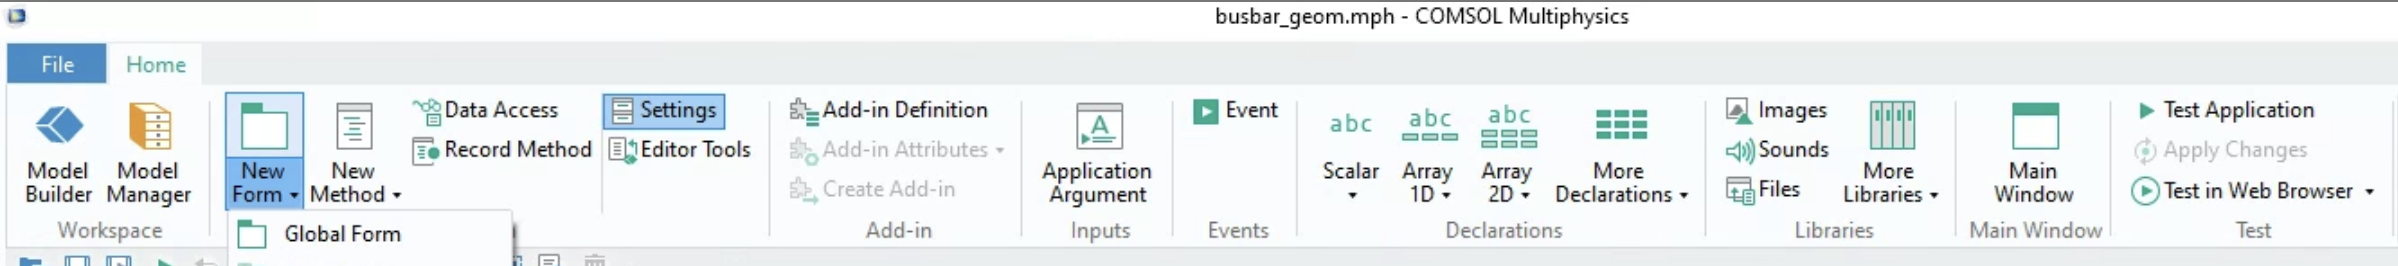
\includegraphics[width=0.7\textwidth]{Chapters/Figures/Chapter 3 Figures/New Form Wizard Button.png}
    \caption{New Form Wizard button. Source: \cite{multiphysics__modeling_nodate}}
    \label{fig:New Form Wizard button}
\end{figure}

After selecting the adjustable parameters, I then focus on the graphical output that will be displayed in the application and ensure that the user interface includes a `Compute Study' button to trigger the simulations.

\begin{figure}[H]
    \centering
    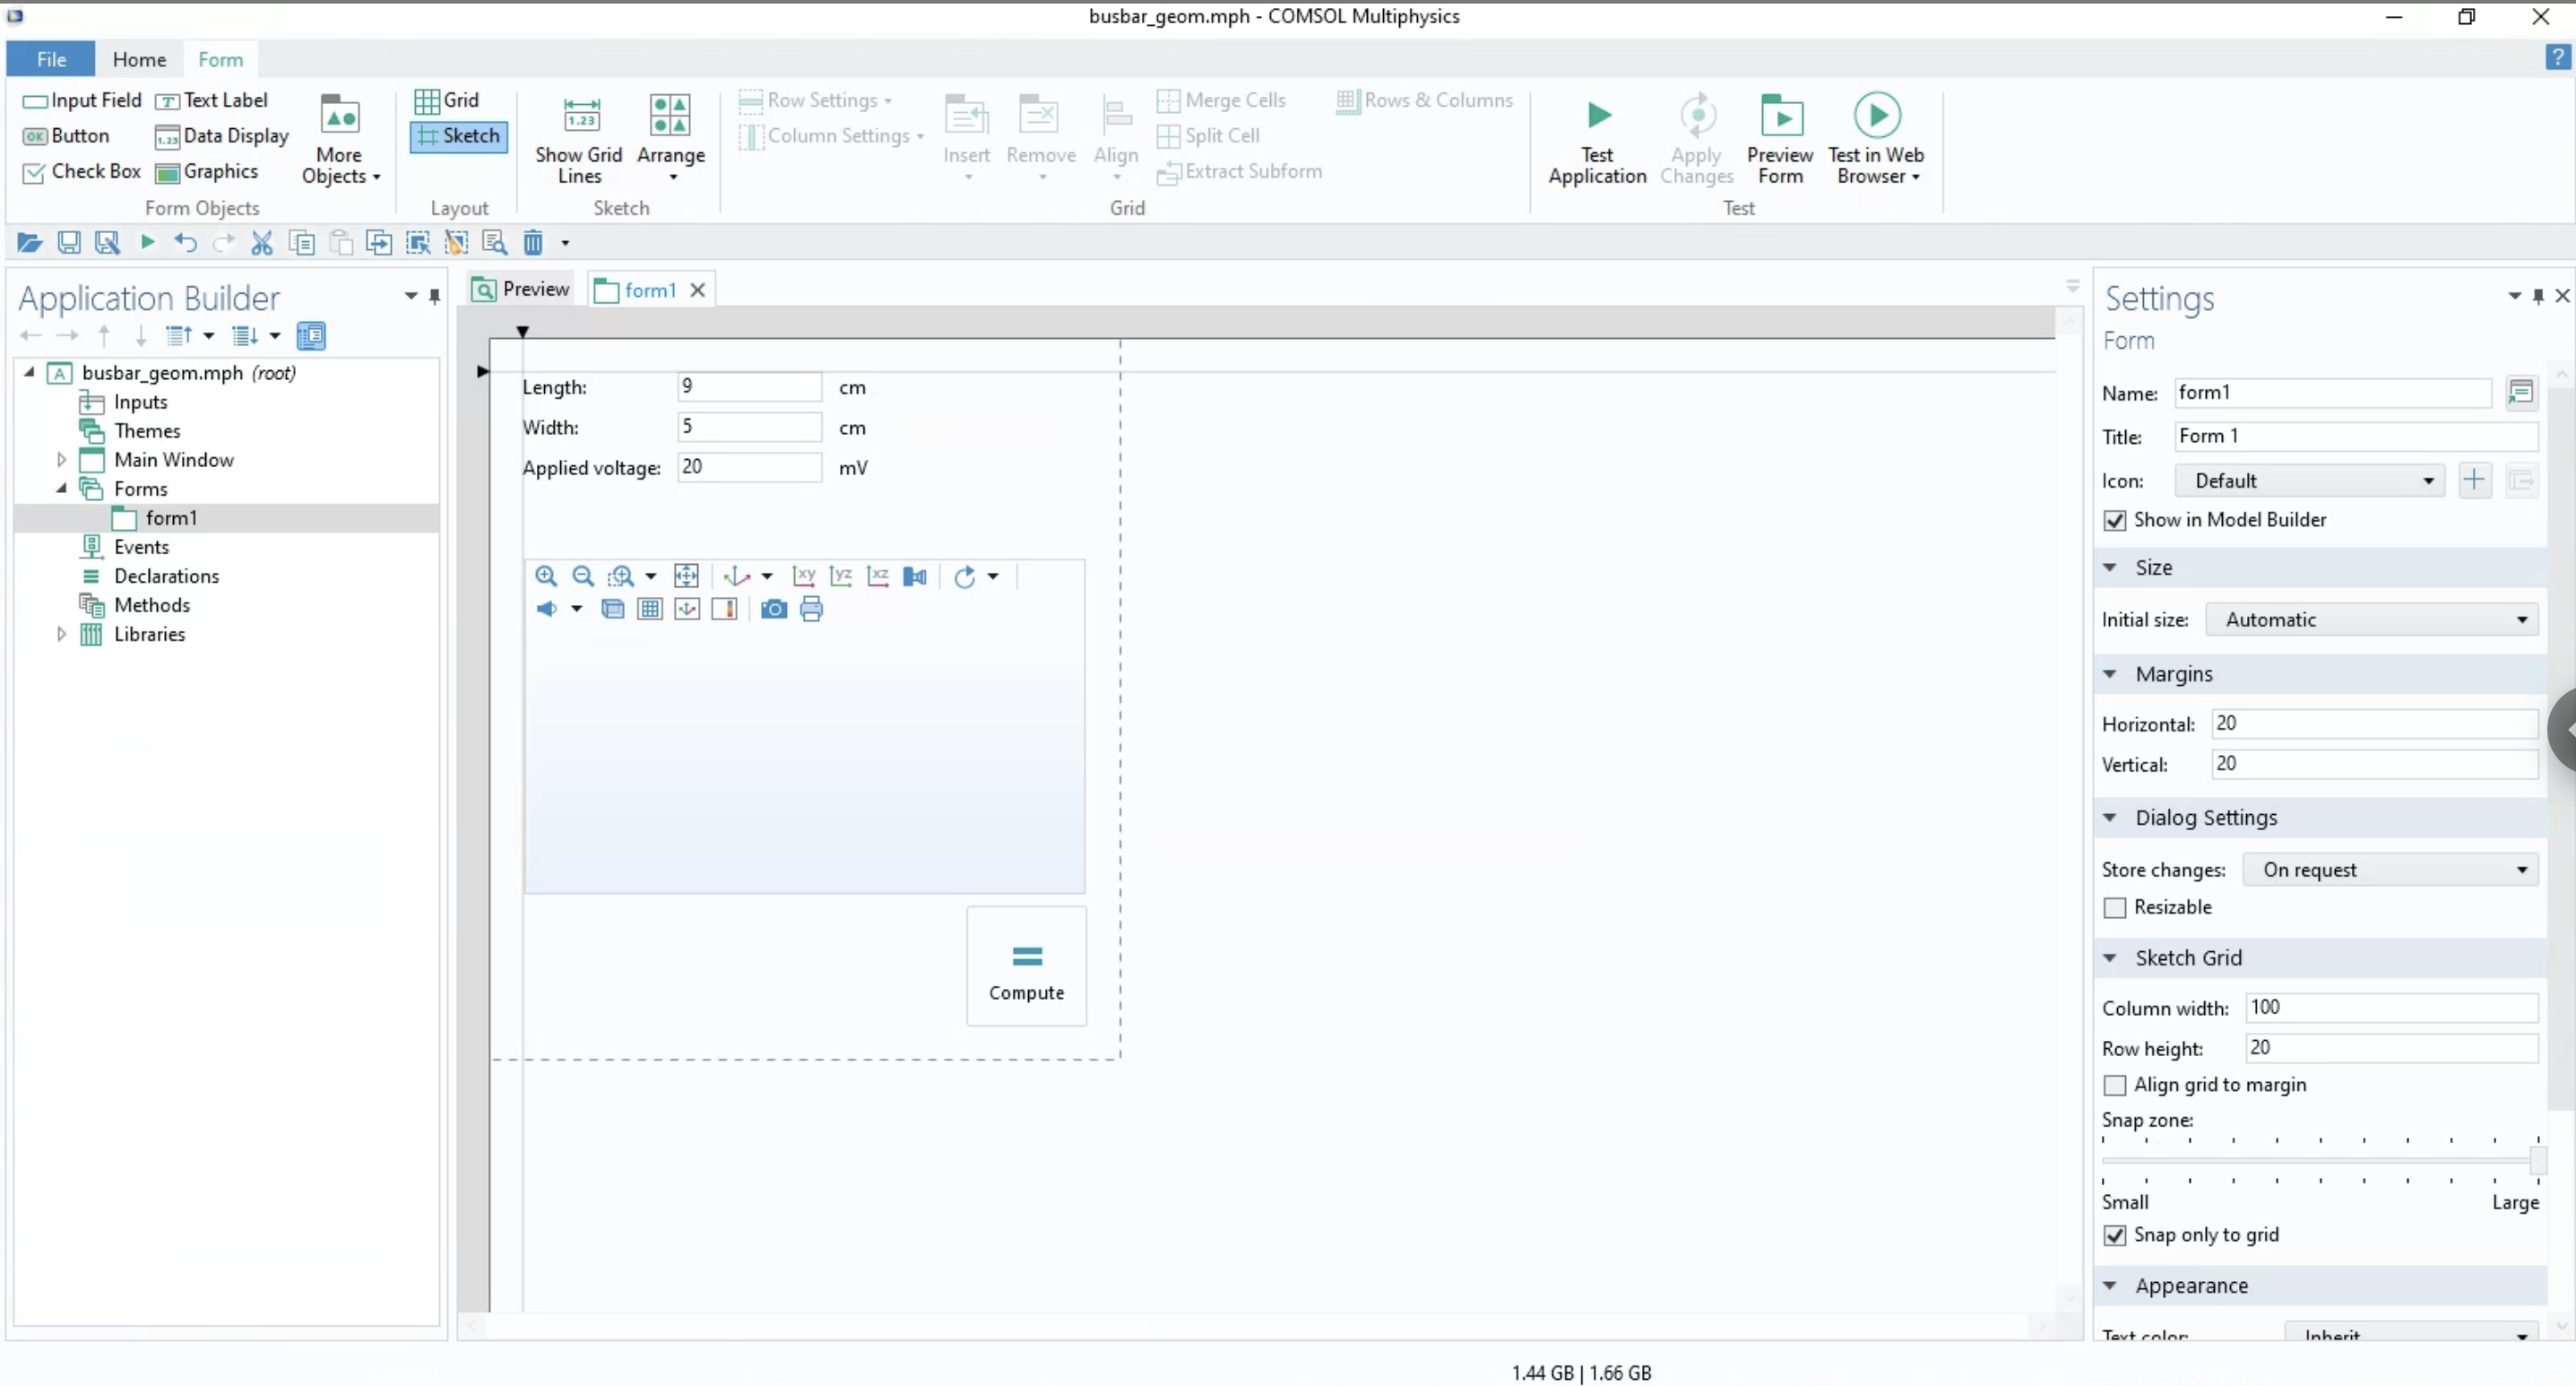
\includegraphics[width=0.7\textwidth]{Chapters/Figures/Chapter 3 Figures/Form Editor Desktop.png}
    \caption{Form Editor. Source: \cite{multiphysics__modeling_nodate}}
    \label{fig:Form Editor}
\end{figure}

Finalizing the interface through the Form Editor allows me to tailor the application's appearance and functionality to meet user needs. This step is crucial for creating a practical tool that can present complex simulations in an approachable manner.

\begin{figure}[H]
    \centering
    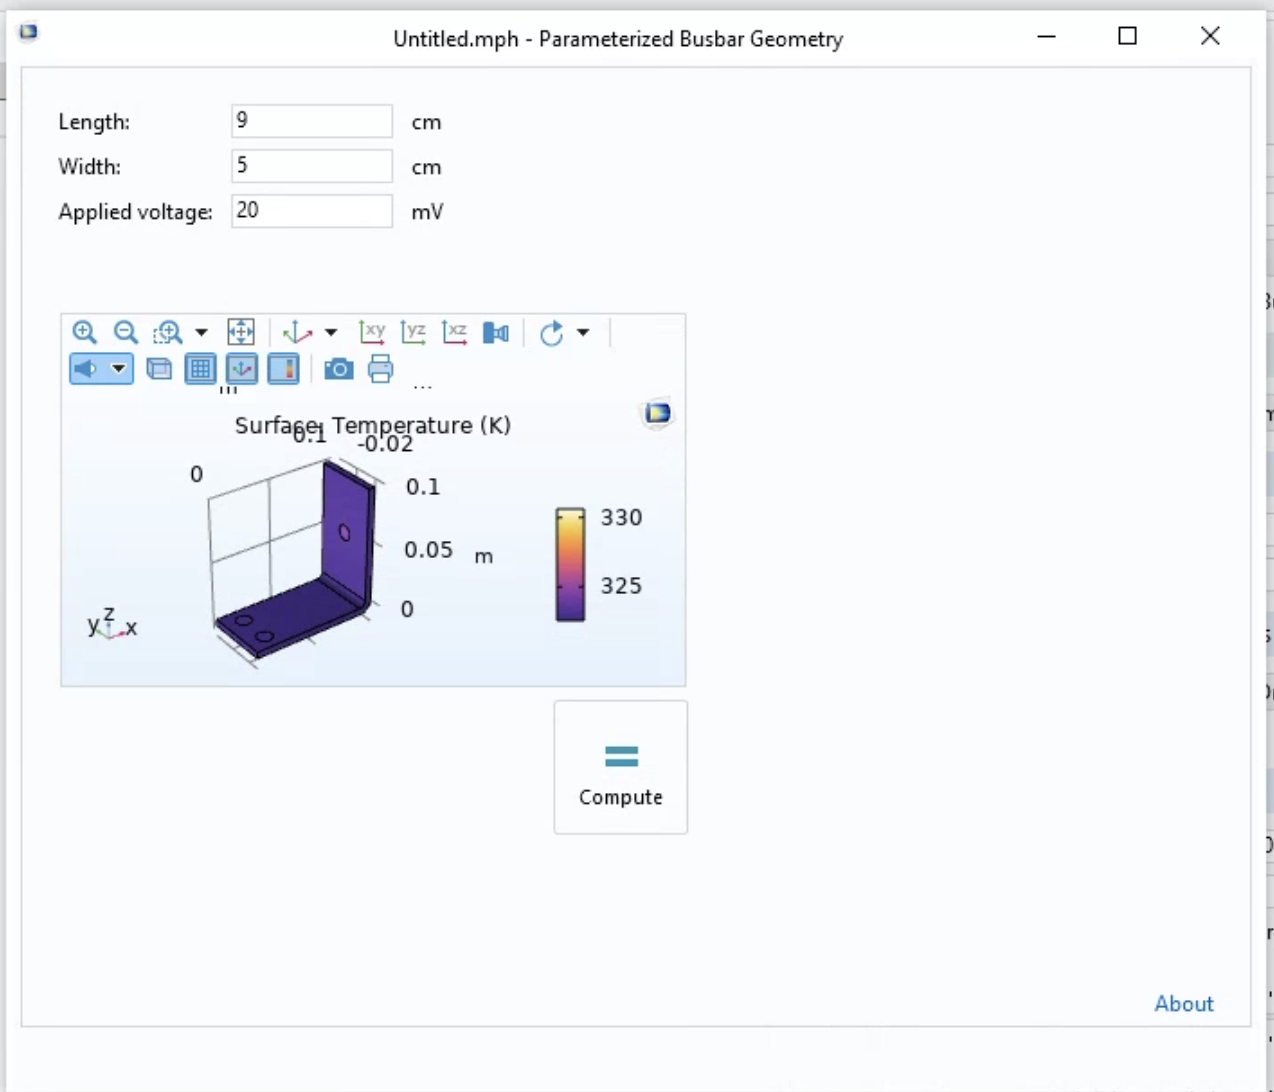
\includegraphics[width=0.7\textwidth]{Chapters/Figures/Chapter 3 Figures/Test Application Results.png}
    \caption{Test Application results. Source: \cite{multiphysics__modeling_nodate}}
    \label{fig:Test Application results}
\end{figure}

In summary, this chapter outlines a comprehensive guide to the computational methods employed in this thesis, using COMSOL Multiphysics™ to model and simulate the behavior of optical systems. The detailed workflow, from initializing the model environment to post-processing the results, demonstrates the capability of COMSOL to handle complex multi-physics problems with a user-friendly approach.

Through the application of this workflow, this chapter not only illustrates the modeling of a busbar to simulate Joule heating but also showcases the customization of the application interface, facilitating accessibility for a broader audience.
